\documentclass[12pt]{report}

\usepackage[utf8]{inputenc}
\usepackage[T1]{fontenc}
\usepackage[spanish]{babel}
\usepackage[a4paper,margin=2.5cm]{geometry}
\usepackage{graphicx}
\usepackage{amsmath}
\usepackage{amssymb}
\usepackage{booktabs}
\usepackage{array}
\usepackage{tabularx}
\usepackage{float}
\usepackage{hyperref}
\usepackage{xcolor}
\usepackage{enumitem}
\usepackage{caption}

\graphicspath{{../outputs/figuras/}}

\hypersetup{
  colorlinks=true,
  linkcolor=blue!50!black,
  urlcolor=blue!50!black
}

\setlist[itemize]{itemsep=0.35em}
\setlength{\parskip}{0.5em}
\setlength{\parindent}{0pt}

\newcommand{\NRPolicy}{\texttt{keep\_current}}
\newcommand{\CurrentValue}{327.223297}
\newcommand{\ExpectedValue}{344.088878}
\newcommand{\ExpectedLoss}{-16.865581}
\newcommand{\PortfolioVol}{21.879552}
\newcommand{\PortfolioVaR}{72.290000}
\newcommand{\PortfolioES}{89.492177}
\newcommand{\LowerTail}{254.930000}
\newcommand{\SupportConv}{3889}
\newcommand{\SupportBrute}{5832}
\newcommand{\ThresholdScenario}{A- | D | CCC}

\title{Tarea CreditMetrics}
\author{Proyecto en Python con validaci\'on exacta por convoluci\'on y \textit{brute force}}
\date{08 de abril de 2026}

\begin{document}

\begin{titlepage}
\centering
{\Huge Tarea CreditMetrics\par}
\vspace{0.7cm}
{\Large Portafolio de 3 bonos independientes\par}
\vspace{1.2cm}
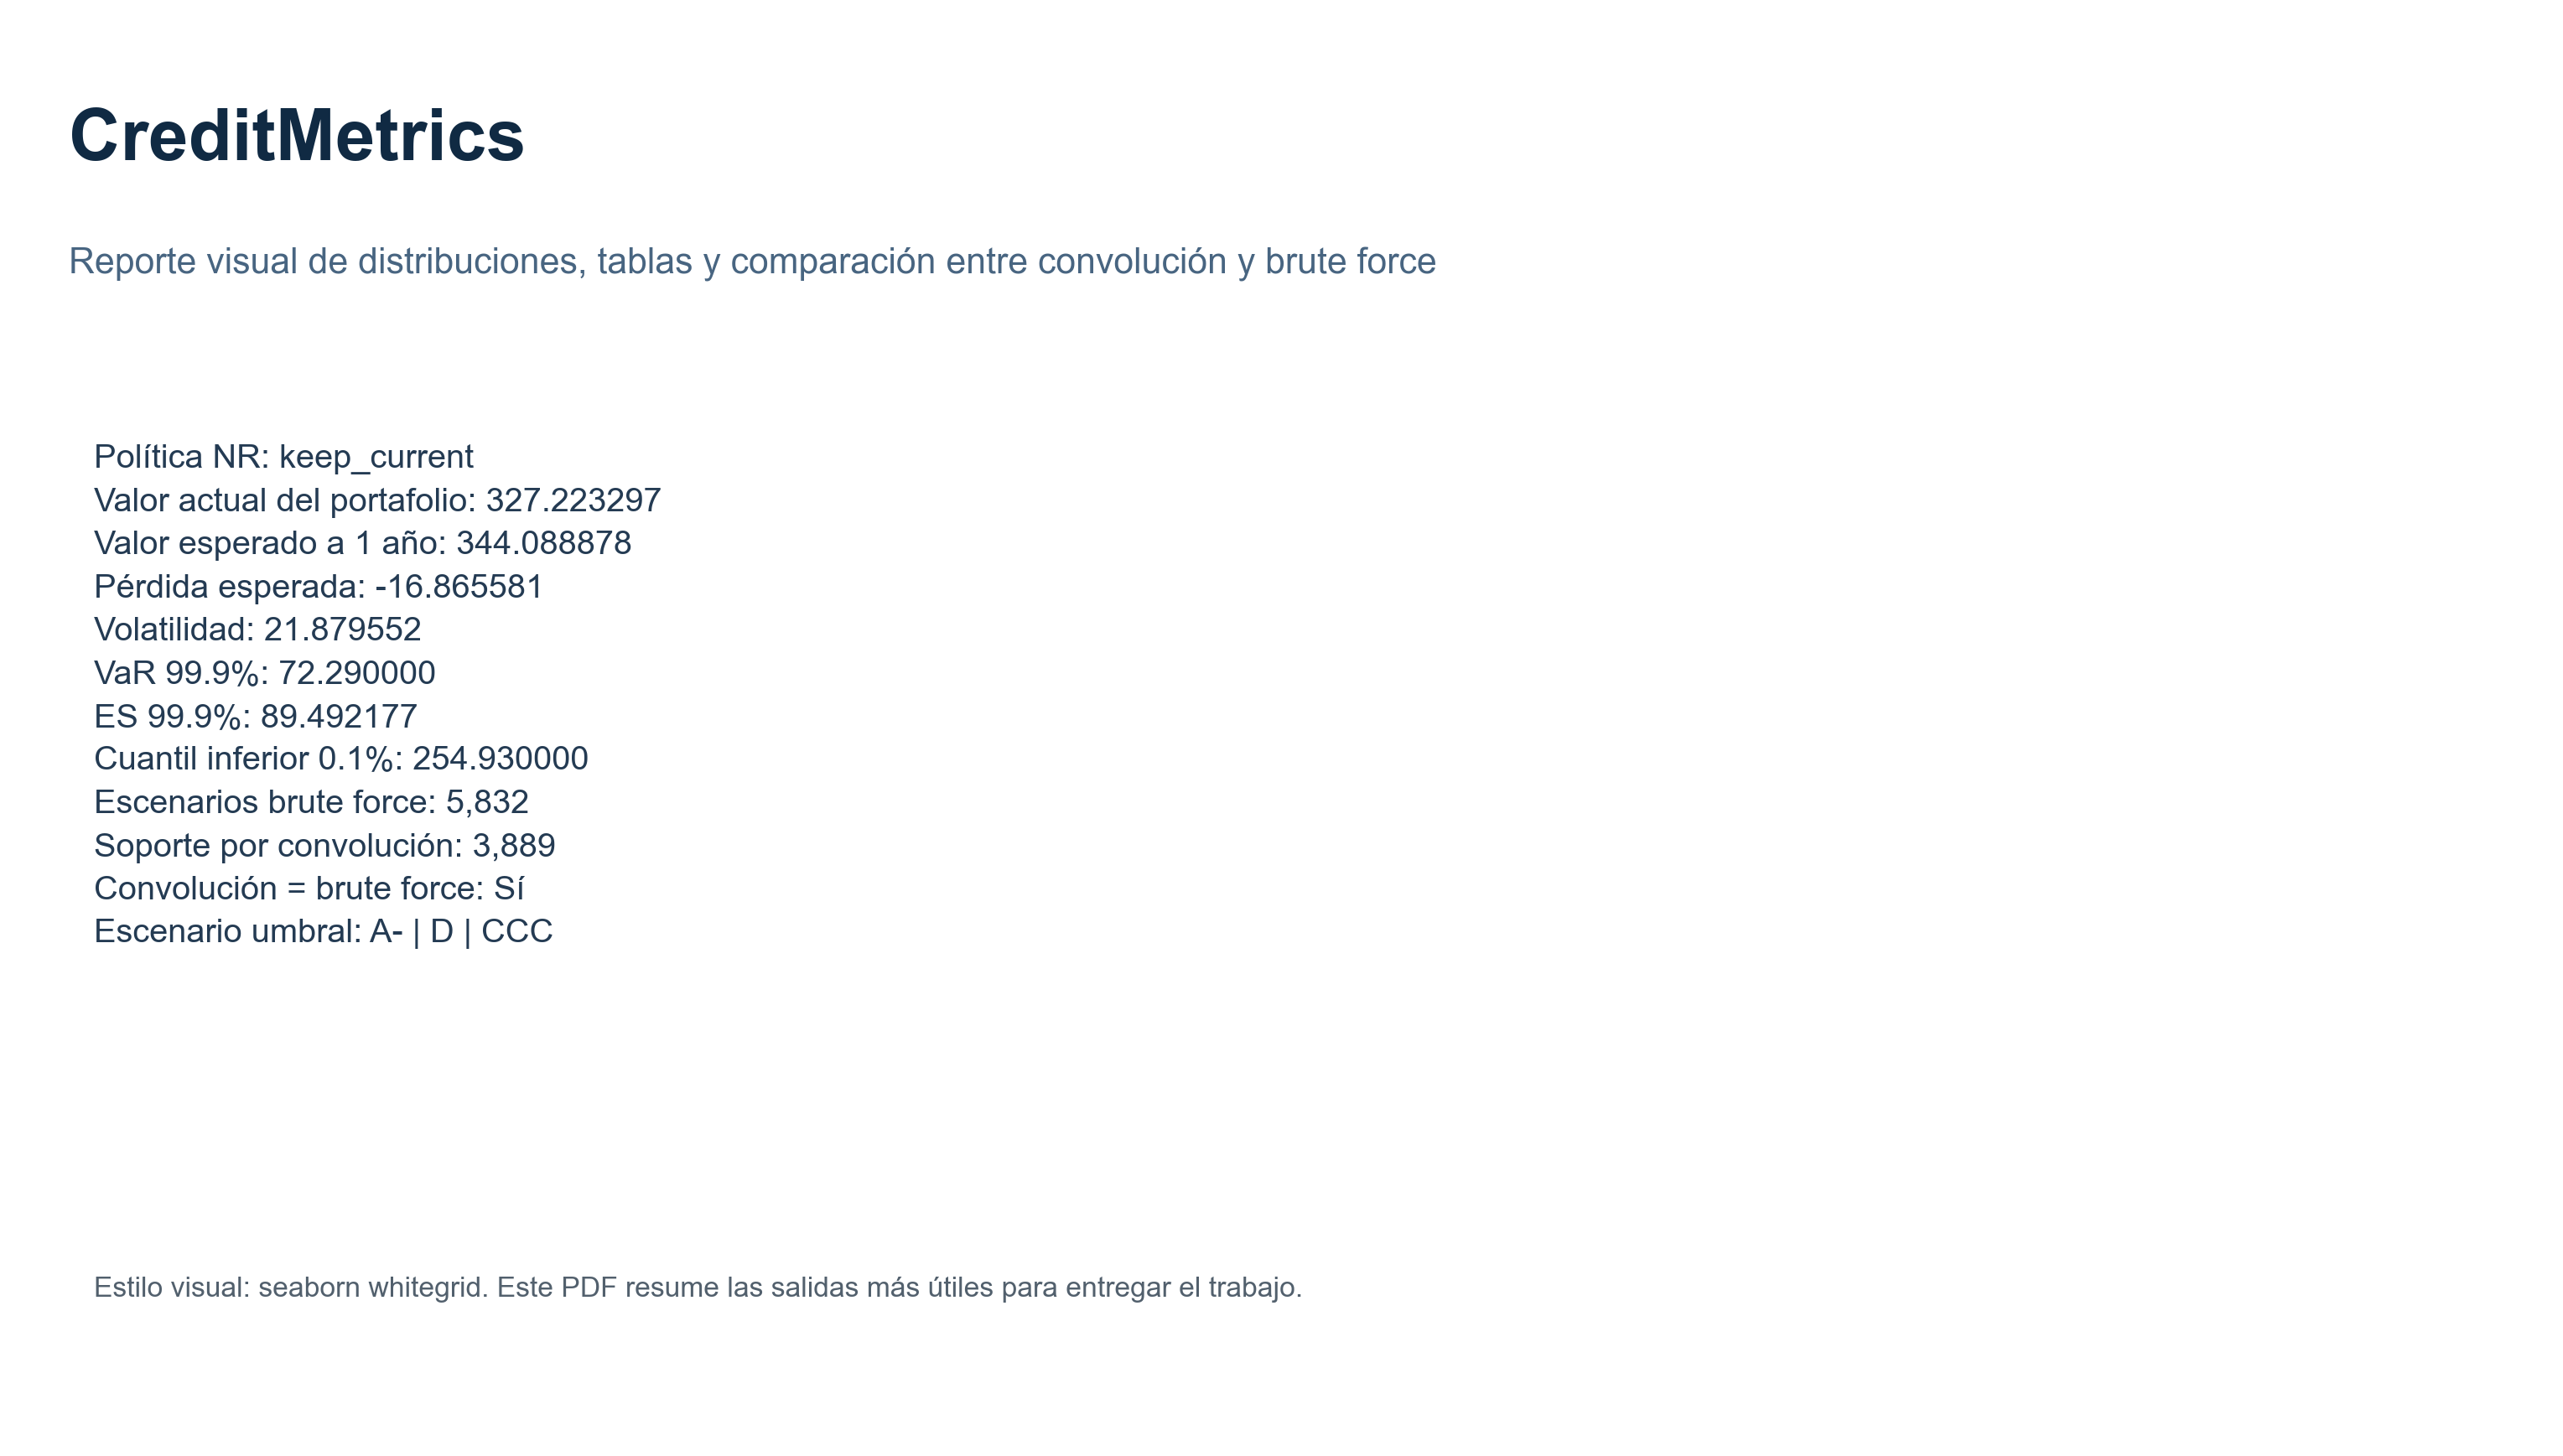
\includegraphics[width=0.95\textwidth]{00_portada_resumen.png}\par
\vspace{1.0cm}
\vfill
\begin{tabular}{>{\bfseries}l l}
Pol\'itica NR usada en la corrida actual: & \NRPolicy \\
Valor actual del portafolio: & \CurrentValue \\
Valor esperado a 1 a\~no: & \ExpectedValue \\
VaR 99.9\%: & \PortfolioVaR \\
ES 99.9\%: & \PortfolioES \\
\end{tabular}
\vfill
{\large 08 de abril de 2026\par}
\end{titlepage}

\pagenumbering{roman}
\tableofcontents
\clearpage
\pagenumbering{arabic}

\chapter{Objetivo del proyecto}
Este proyecto resuelve un ejercicio de \textit{CreditMetrics} para un portafolio compuesto por tres bonos corporativos independientes con calificaciones iniciales A-, BBB- y B-. Cada bono tiene vencimiento original de 5 a\~nos y se analiza en un horizonte de riesgo de 1 a\~no.

La idea central del repositorio es evitar una tabla manual de los \(18^3 = 5{,}832\) escenarios posibles. En lugar de eso, el c\'odigo:

\begin{itemize}
  \item calcula la distribuci\'on discreta de valor a 1 a\~no de cada bono;
  \item comprime esa distribuci\'on a centavos;
  \item construye la distribuci\'on del portafolio mediante convoluci\'on exacta;
  \item valida el resultado contra una enumeraci\'on \textit{brute force} de todos los escenarios;
  \item exporta resultados en CSV, JSON, Excel, im\'agenes PNG y PDF.
\end{itemize}

La corrida actual del proyecto usa la pol\'itica \NRPolicy\ para la columna \texttt{NR}. Bajo esa pol\'itica, la masa de \texttt{NR} se asigna al rating actual de cada bono.

El objetivo pr\'actico del c\'odigo no es solo producir un VaR, sino dejar trazabilidad completa del proceso: datos base, valuaci\'on por estado, distribuciones marginales, comparaci\'on convoluci\'on vs \textit{brute force} y material visual listo para entregar.


\chapter{Arquitectura y flujo del c\'odigo}
El proyecto est\'a organizado de manera simple y funcional. Los archivos principales son:

\begin{itemize}
  \item \texttt{src/creditmetrics\_project/data.py}: concentra los insumos del ejercicio.
  \item \texttt{src/creditmetrics\_project/model.py}: contiene toda la l\'ogica cuantitativa y de exportaci\'on.
  \item \texttt{src/creditmetrics\_project/main.py}: expone la interfaz de l\'inea de comandos.
\end{itemize}

\section*{Qu\'e hace \texttt{data.py}}

En este archivo se definen:

\begin{itemize}
  \item el espacio de 18 estados de rating;
  \item la curva libre de riesgo del ejercicio;
  \item los spreads de cr\'edito por rating;
  \item la matriz de transici\'on anual;
  \item la especificaci\'on de los tres bonos del portafolio.
\end{itemize}

Es, en la pr\'actica, la capa de entrada del modelo.

\section*{Qu\'e hace \texttt{model.py}}

Este archivo implementa casi todo el trabajo cuantitativo. Sus bloques m\'as importantes son:

\begin{itemize}
  \item \texttt{price\_bond\_today}: calcula el precio actual de un bono con la curva libre de riesgo m\'as el spread correspondiente a su rating.
  \item \texttt{price\_bond\_at\_horizon\_given\_state}: calcula el valor del bono a 1 a\~no, condicionado al estado migrado.
  \item \texttt{normalized\_transition\_row}: ajusta la fila de probabilidades seg\'un la pol\'itica aplicada a \texttt{NR}.
  \item \texttt{single\_bond\_distribution}: genera la distribuci\'on discreta de cada bono.
  \item \texttt{compress\_distribution\_to\_cents}: agrupa valores a nivel centavos para poder convolucionar una PMF discreta limpia.
  \item \texttt{convolve\_pmfs}: suma distribuciones discretas independientes.
  \item \texttt{portfolio\_distribution\_bruteforce}: enumera los \(5{,}832\) escenarios posibles y sirve de validaci\'on exacta.
  \item \texttt{write\_outputs}: exporta CSV, JSON, Excel, gr\'aficas e informe visual.
\end{itemize}

\section*{Qu\'e hace \texttt{main.py}}

El archivo principal recibe los argumentos de ejecuci\'on, lanza \texttt{run\_analysis} y muestra en consola un resumen del portafolio y de cada bono.

\section*{Flujo operativo}

El flujo completo del programa es el siguiente:

\begin{enumerate}
  \item cargar datos del ejercicio;
  \item valuar el precio actual de cada bono;
  \item construir la distribuci\'on de valor a 1 a\~no por bono;
  \item resumir media, volatilidad y VaR individual;
  \item convolucionar las tres distribuciones;
  \item construir la PMF del portafolio por \textit{brute force};
  \item comparar ambos resultados;
  \item exportar tablas y reportes.
\end{enumerate}

La decisi\'on de separar datos, l\'ogica y CLI vuelve al repositorio f\'acil de modificar. Por ejemplo, si cambia la pol\'itica \texttt{NR}, la curva libre de riesgo o el conjunto de bonos, no hace falta reescribir el flujo general.


\chapter{Metodolog\'ia implementada}
La l\'ogica financiera del c\'odigo sigue la estructura cl\'asica de CreditMetrics para bonos con cupones anuales.

\section*{1. Precio actual}

Para cada bono se calcula primero su precio actual:

\[
P_0 = \sum_{t=1}^{T-1}\frac{C}{(1+y_t)^t} + \frac{C+N}{(1+y_T)^T},
\]

donde \(C\) es el cup\'on, \(N\) es el valor nominal y \(y_t\) combina la curva libre de riesgo con el spread del rating actual.

\section*{2. Valor al horizonte condicionado al estado}

En el horizonte de 1 a\~no, el modelo distingue dos casos:

\begin{itemize}
  \item si el bono no entra en default, se recibe el cup\'on del a\~no 1 y luego se reval\'ua el bono remanente con vencimiento residual de 4 a\~nos;
  \item si el bono migra a \(D\), se usa el valor de recuperaci\'on definido en el ejercicio.
\end{itemize}

Para un estado migrado \(r \neq D\), el valor al horizonte es:

\[
V_1(r)=C+\sum_{u=1}^{3}\frac{C}{(1+y_u(r))^u}+\frac{C+N}{(1+y_4(r))^4}.
\]

\section*{3. Distribuci\'on discreta por bono}

Una vez que se tiene el valor \(V_1(r)\) para cada uno de los 18 estados, se asigna a cada estado su probabilidad de migraci\'on. Esto produce una distribuci\'on discreta del valor del bono a 1 a\~no.

\section*{4. Compresi\'on a centavos}

El c\'odigo agrupa los valores a nivel centavos. Esa decisi\'on tiene dos ventajas:

\begin{itemize}
  \item reduce el tama\~no del soporte de la distribuci\'on;
  \item permite una convoluci\'on exacta sobre una PMF discreta ordenada.
\end{itemize}

La funci\'on \texttt{compress\_distribution\_to\_cents} es clave para este paso.

\section*{5. Convoluci\'on del portafolio}

Si \(X_1\), \(X_2\) y \(X_3\) son las distribuciones de los tres bonos, la del portafolio es:

\[
X_P = X_1 + X_2 + X_3.
\]

Bajo independencia:

\[
\mathbb{P}(X_P=v)=\left(\mathbb{P}_{X_1} * \mathbb{P}_{X_2} * \mathbb{P}_{X_3}\right)(v).
\]

Esto permite construir la PMF del portafolio sin crear manualmente toda la tabla de escenarios.

\section*{6. Validaci\'on por brute force}

Aunque la convoluci\'on es el m\'etodo eficiente, el proyecto calcula tambi\'en la distribuci\'on por enumeraci\'on completa de los \(5{,}832\) escenarios. La PMF resultante se compara contra la de convoluci\'on.

La corrida actual confirma:

\begin{itemize}
  \item soporte por convoluci\'on: \SupportConv;
  \item escenarios \textit{brute force}: \SupportBrute;
  \item coincidencia entre ambos m\'etodos a nivel centavos.
\end{itemize}

\section*{7. M\'etricas finales}

Con la distribuci\'on final del portafolio, el modelo calcula:

\begin{itemize}
  \item valor esperado a 1 a\~no;
  \item p\'erdida esperada;
  \item volatilidad;
  \item VaR al 99.9\%;
  \item ES al 99.9\%;
  \item cuantil inferior 0.1\% del valor del portafolio.
\end{itemize}

En la corrida actual, los principales resultados del portafolio son:

\begin{center}
\begin{tabular}{lr}
\toprule
M\'etrica & Valor \\
\midrule
Valor actual & \CurrentValue \\
Valor esperado a 1 a\~no & \ExpectedValue \\
P\'erdida esperada & \ExpectedLoss \\
Volatilidad & \PortfolioVol \\
VaR 99.9\% & \PortfolioVaR \\
ES 99.9\% & \PortfolioES \\
Cuantil 0.1\% del valor & \LowerTail \\
\bottomrule
\end{tabular}
\end{center}


\chapter{Resultados y visualizaciones}
Esta secci\'on presenta las salidas visuales generadas por el propio proyecto en Python. Las figuras se insertan directamente desde \texttt{outputs/figuras/}, de modo que el documento queda alineado con la corrida actual.

\section*{Resumen ejecutivo del portafolio}

\begin{figure}[H]
\centering
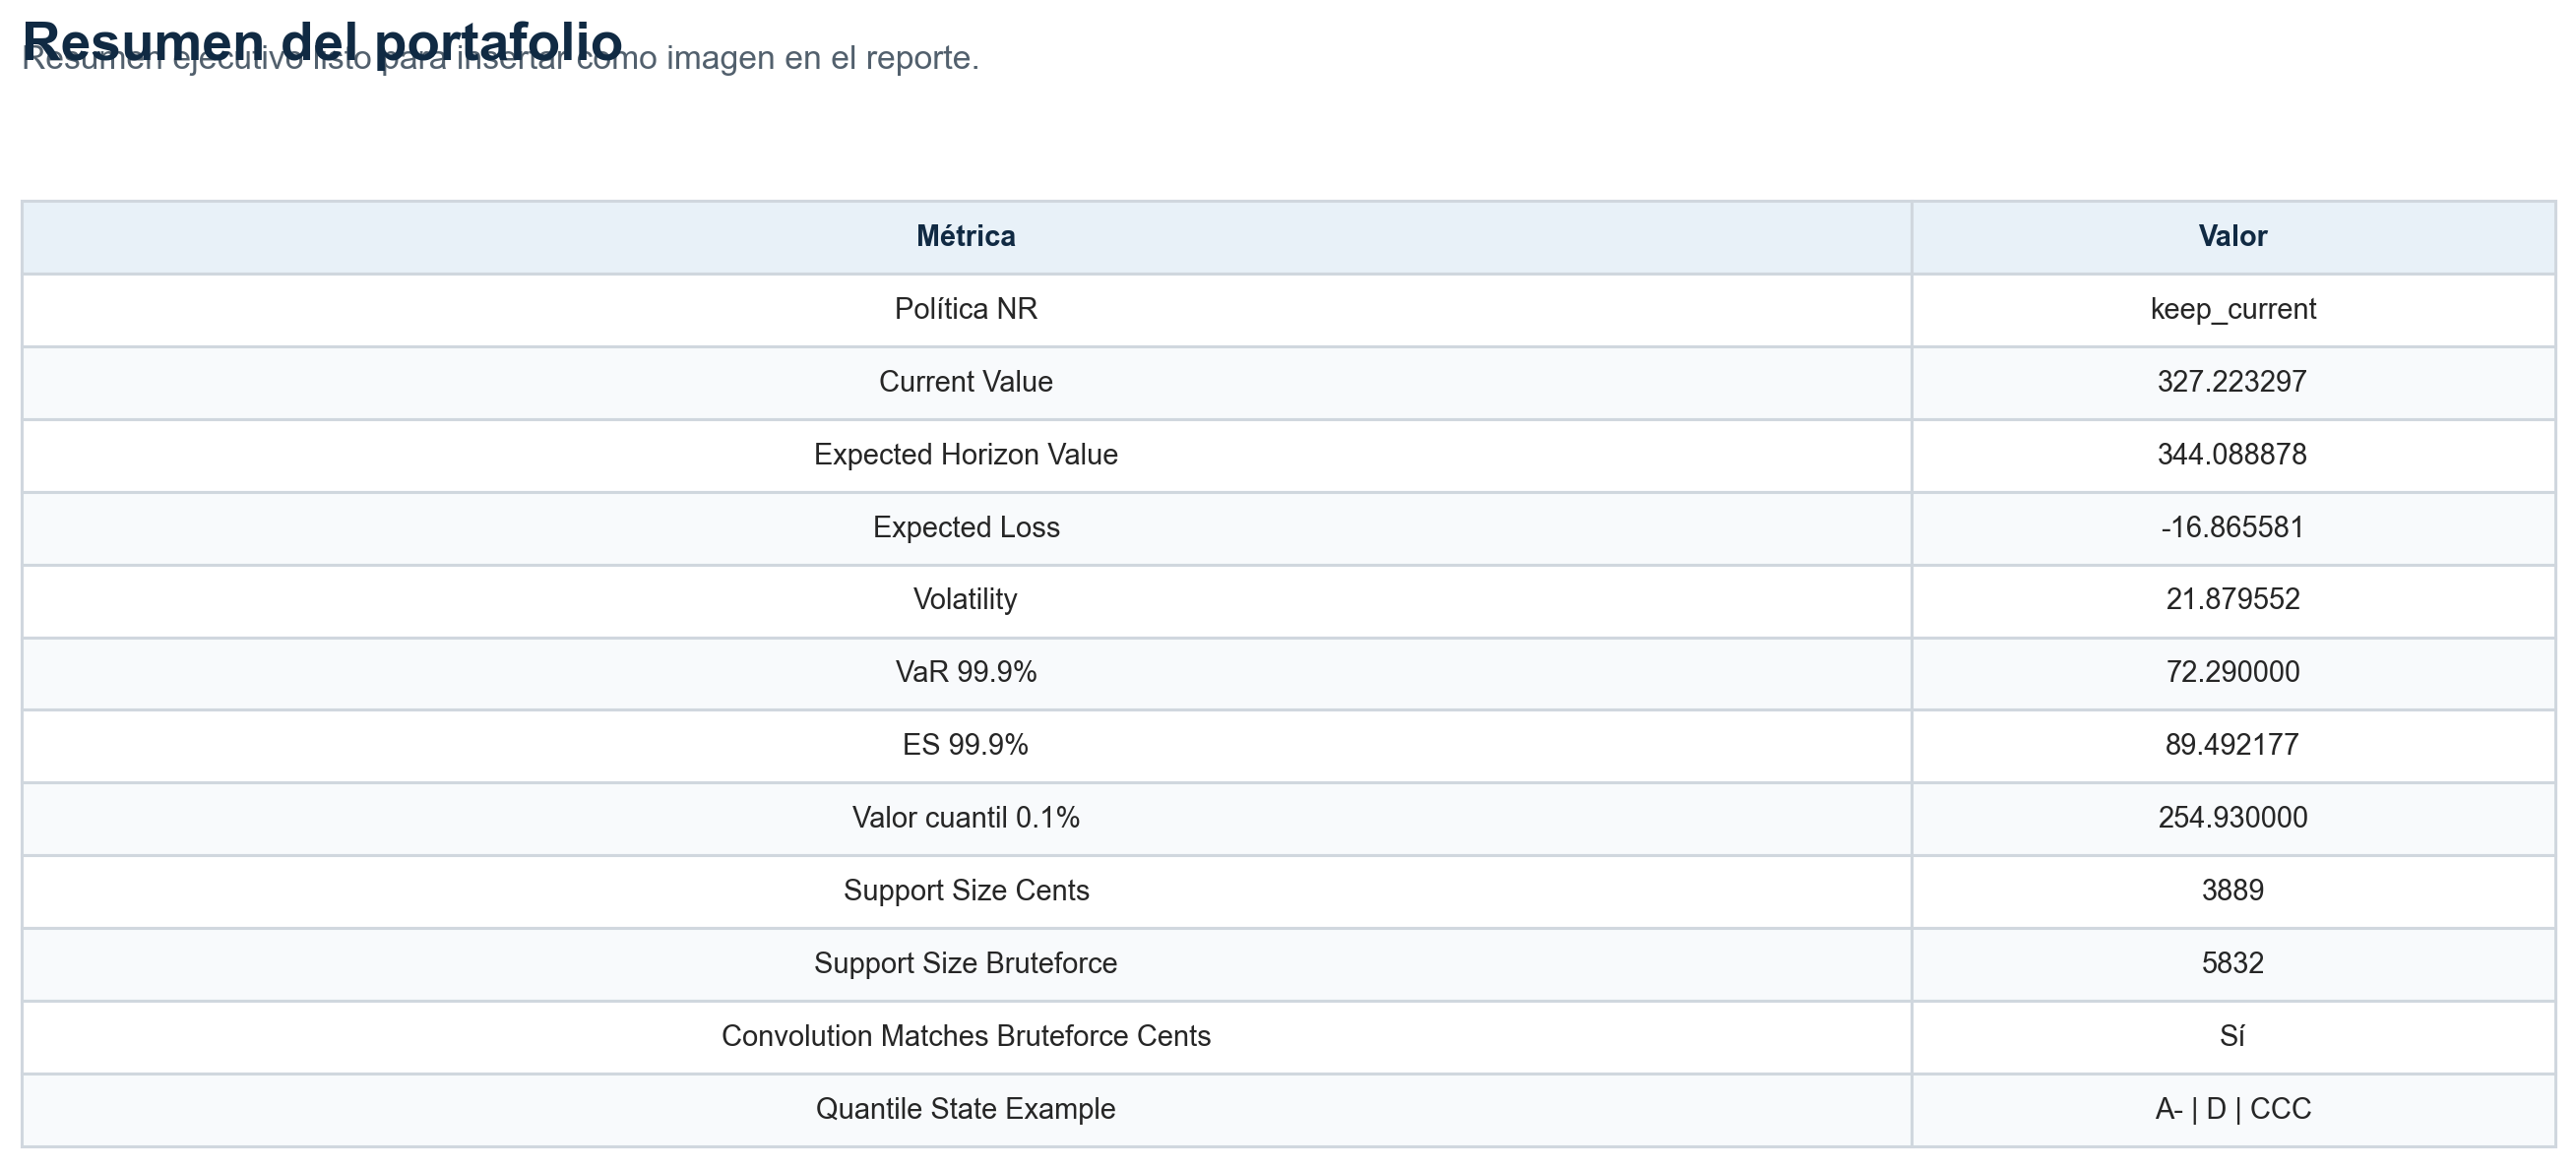
\includegraphics[width=0.95\textwidth]{01_tabla_resumen_portafolio.png}
\caption{Resumen del portafolio para la corrida actual.}
\end{figure}

La tabla anterior resume las magnitudes centrales del ejercicio. El valor esperado a 1 a\~no es mayor que el valor actual, por lo que la p\'erdida esperada aparece con signo negativo. Eso refleja que, en promedio, el efecto de carry y cupones domina a la p\'erdida esperada por migraci\'on crediticia.

\begin{figure}[H]
\centering
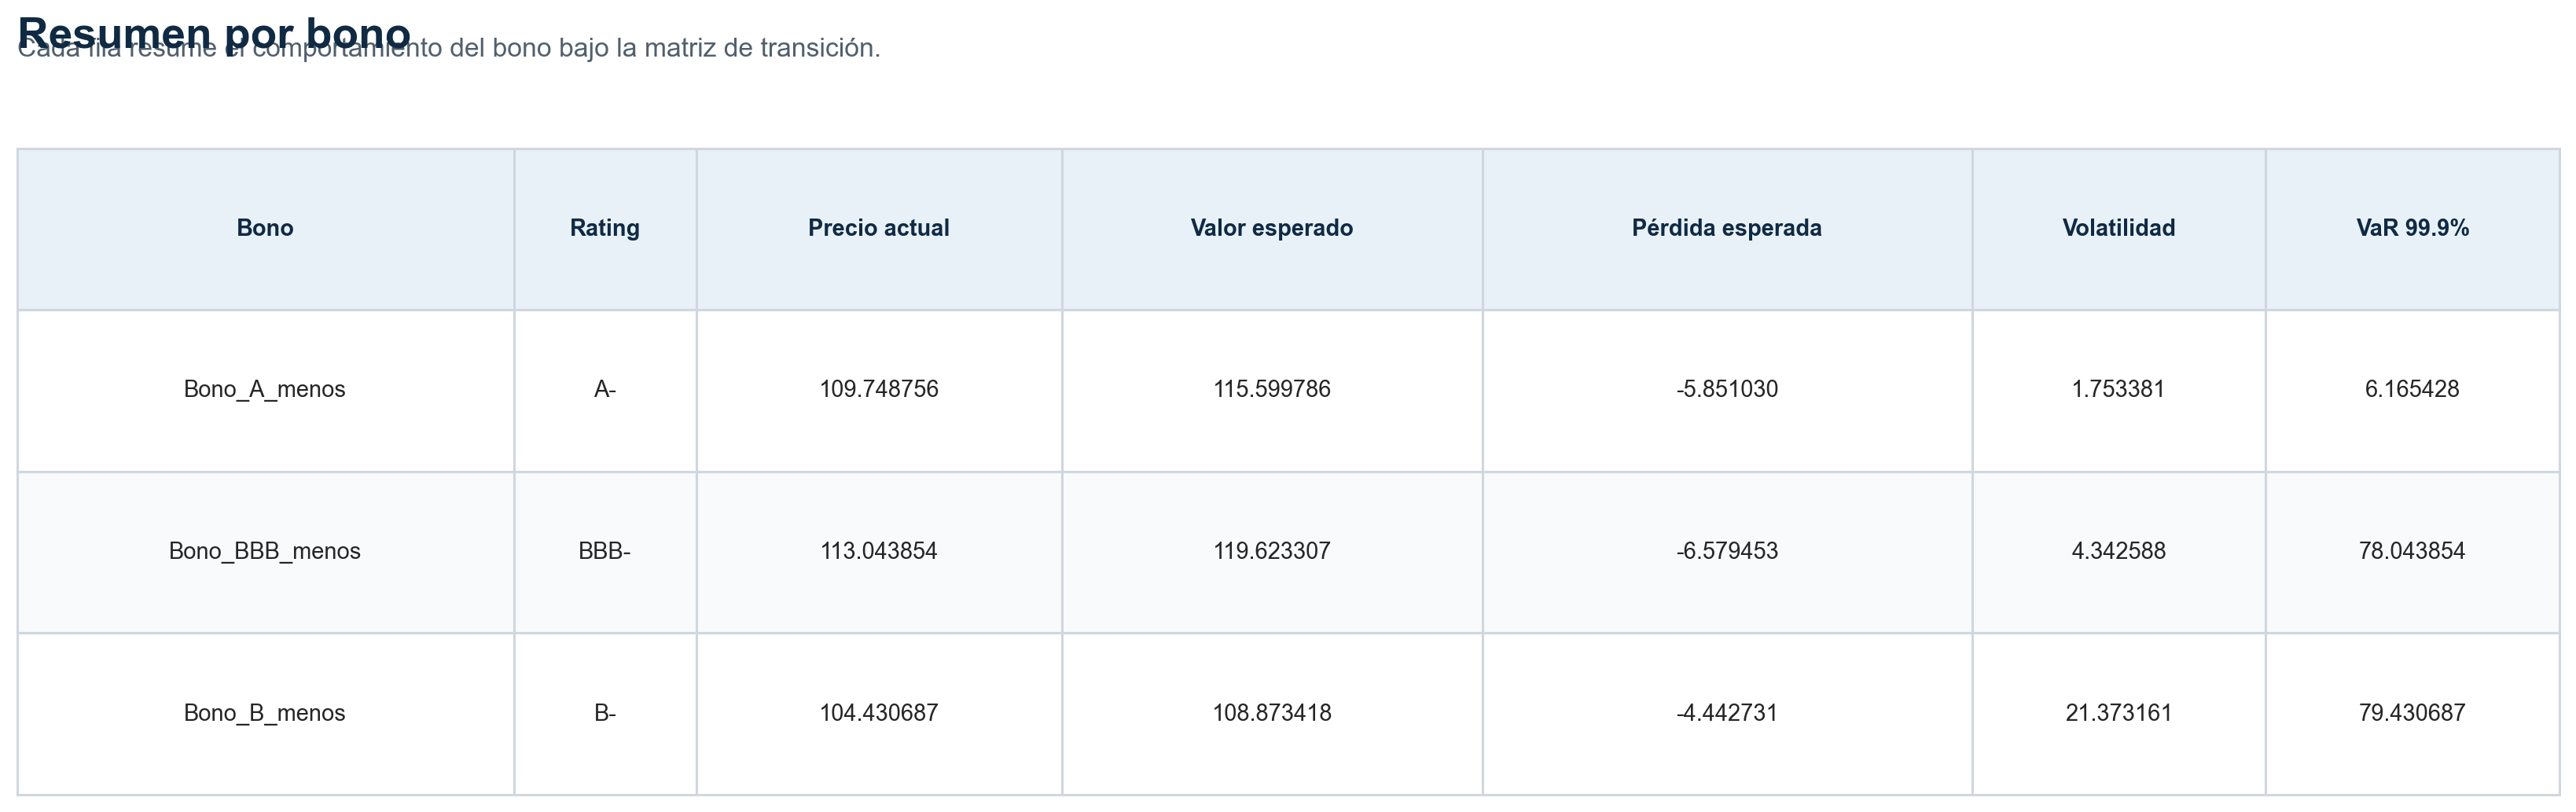
\includegraphics[width=\textwidth]{02_tabla_resumen_bonos.png}
\caption{Resumen comparativo de los tres bonos.}
\end{figure}

La tabla por bono deja ver una diferencia importante en perfil de riesgo: el bono A- es mucho m\'as estable, mientras que los bonos BBB- y B- concentran la mayor parte del riesgo extremo del portafolio.

\section*{Distribuciones marginales por bono}

\begin{figure}[H]
\centering
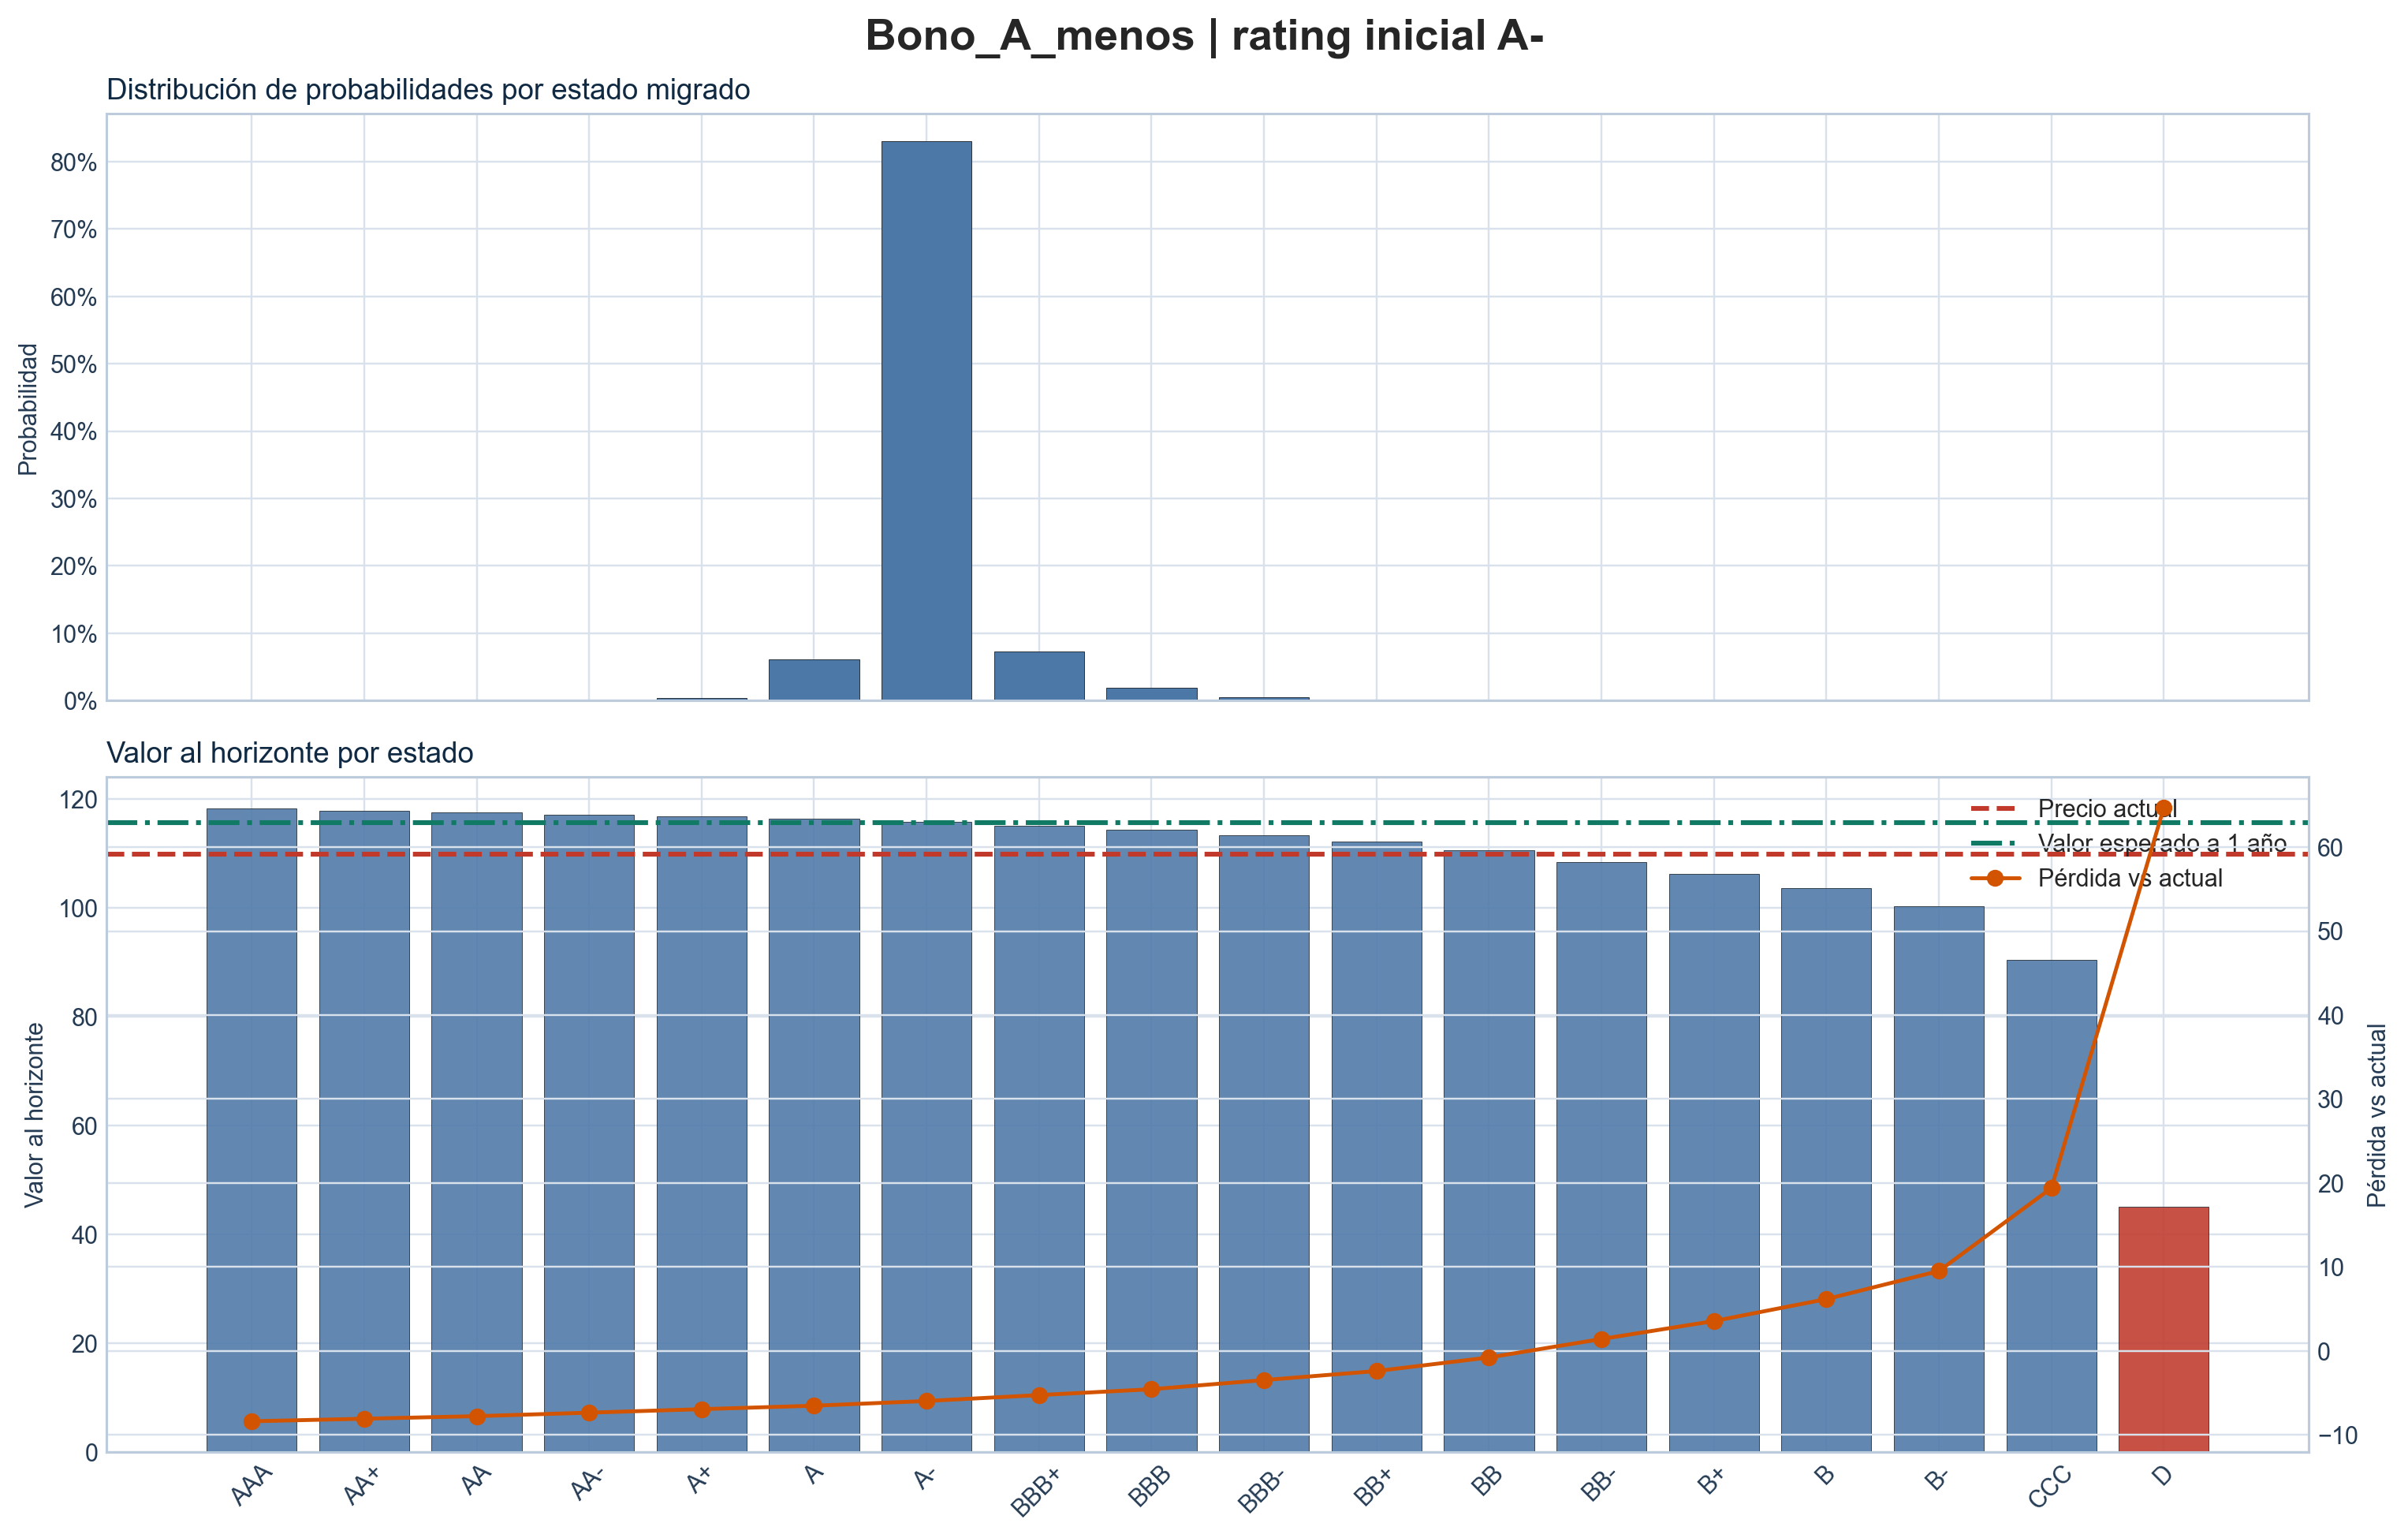
\includegraphics[width=\textwidth]{03_grafica_bono_a_menos.png}
\caption{Distribuci\'on de probabilidad y valor al horizonte para el bono A-.}
\end{figure}

En el bono A-, la masa de probabilidad permanece concentrada en ratings cercanos a su estado inicial. La dispersi\'on del valor al horizonte es baja y el default tiene muy baja probabilidad, por eso su volatilidad es la menor del grupo.

\begin{figure}[H]
\centering
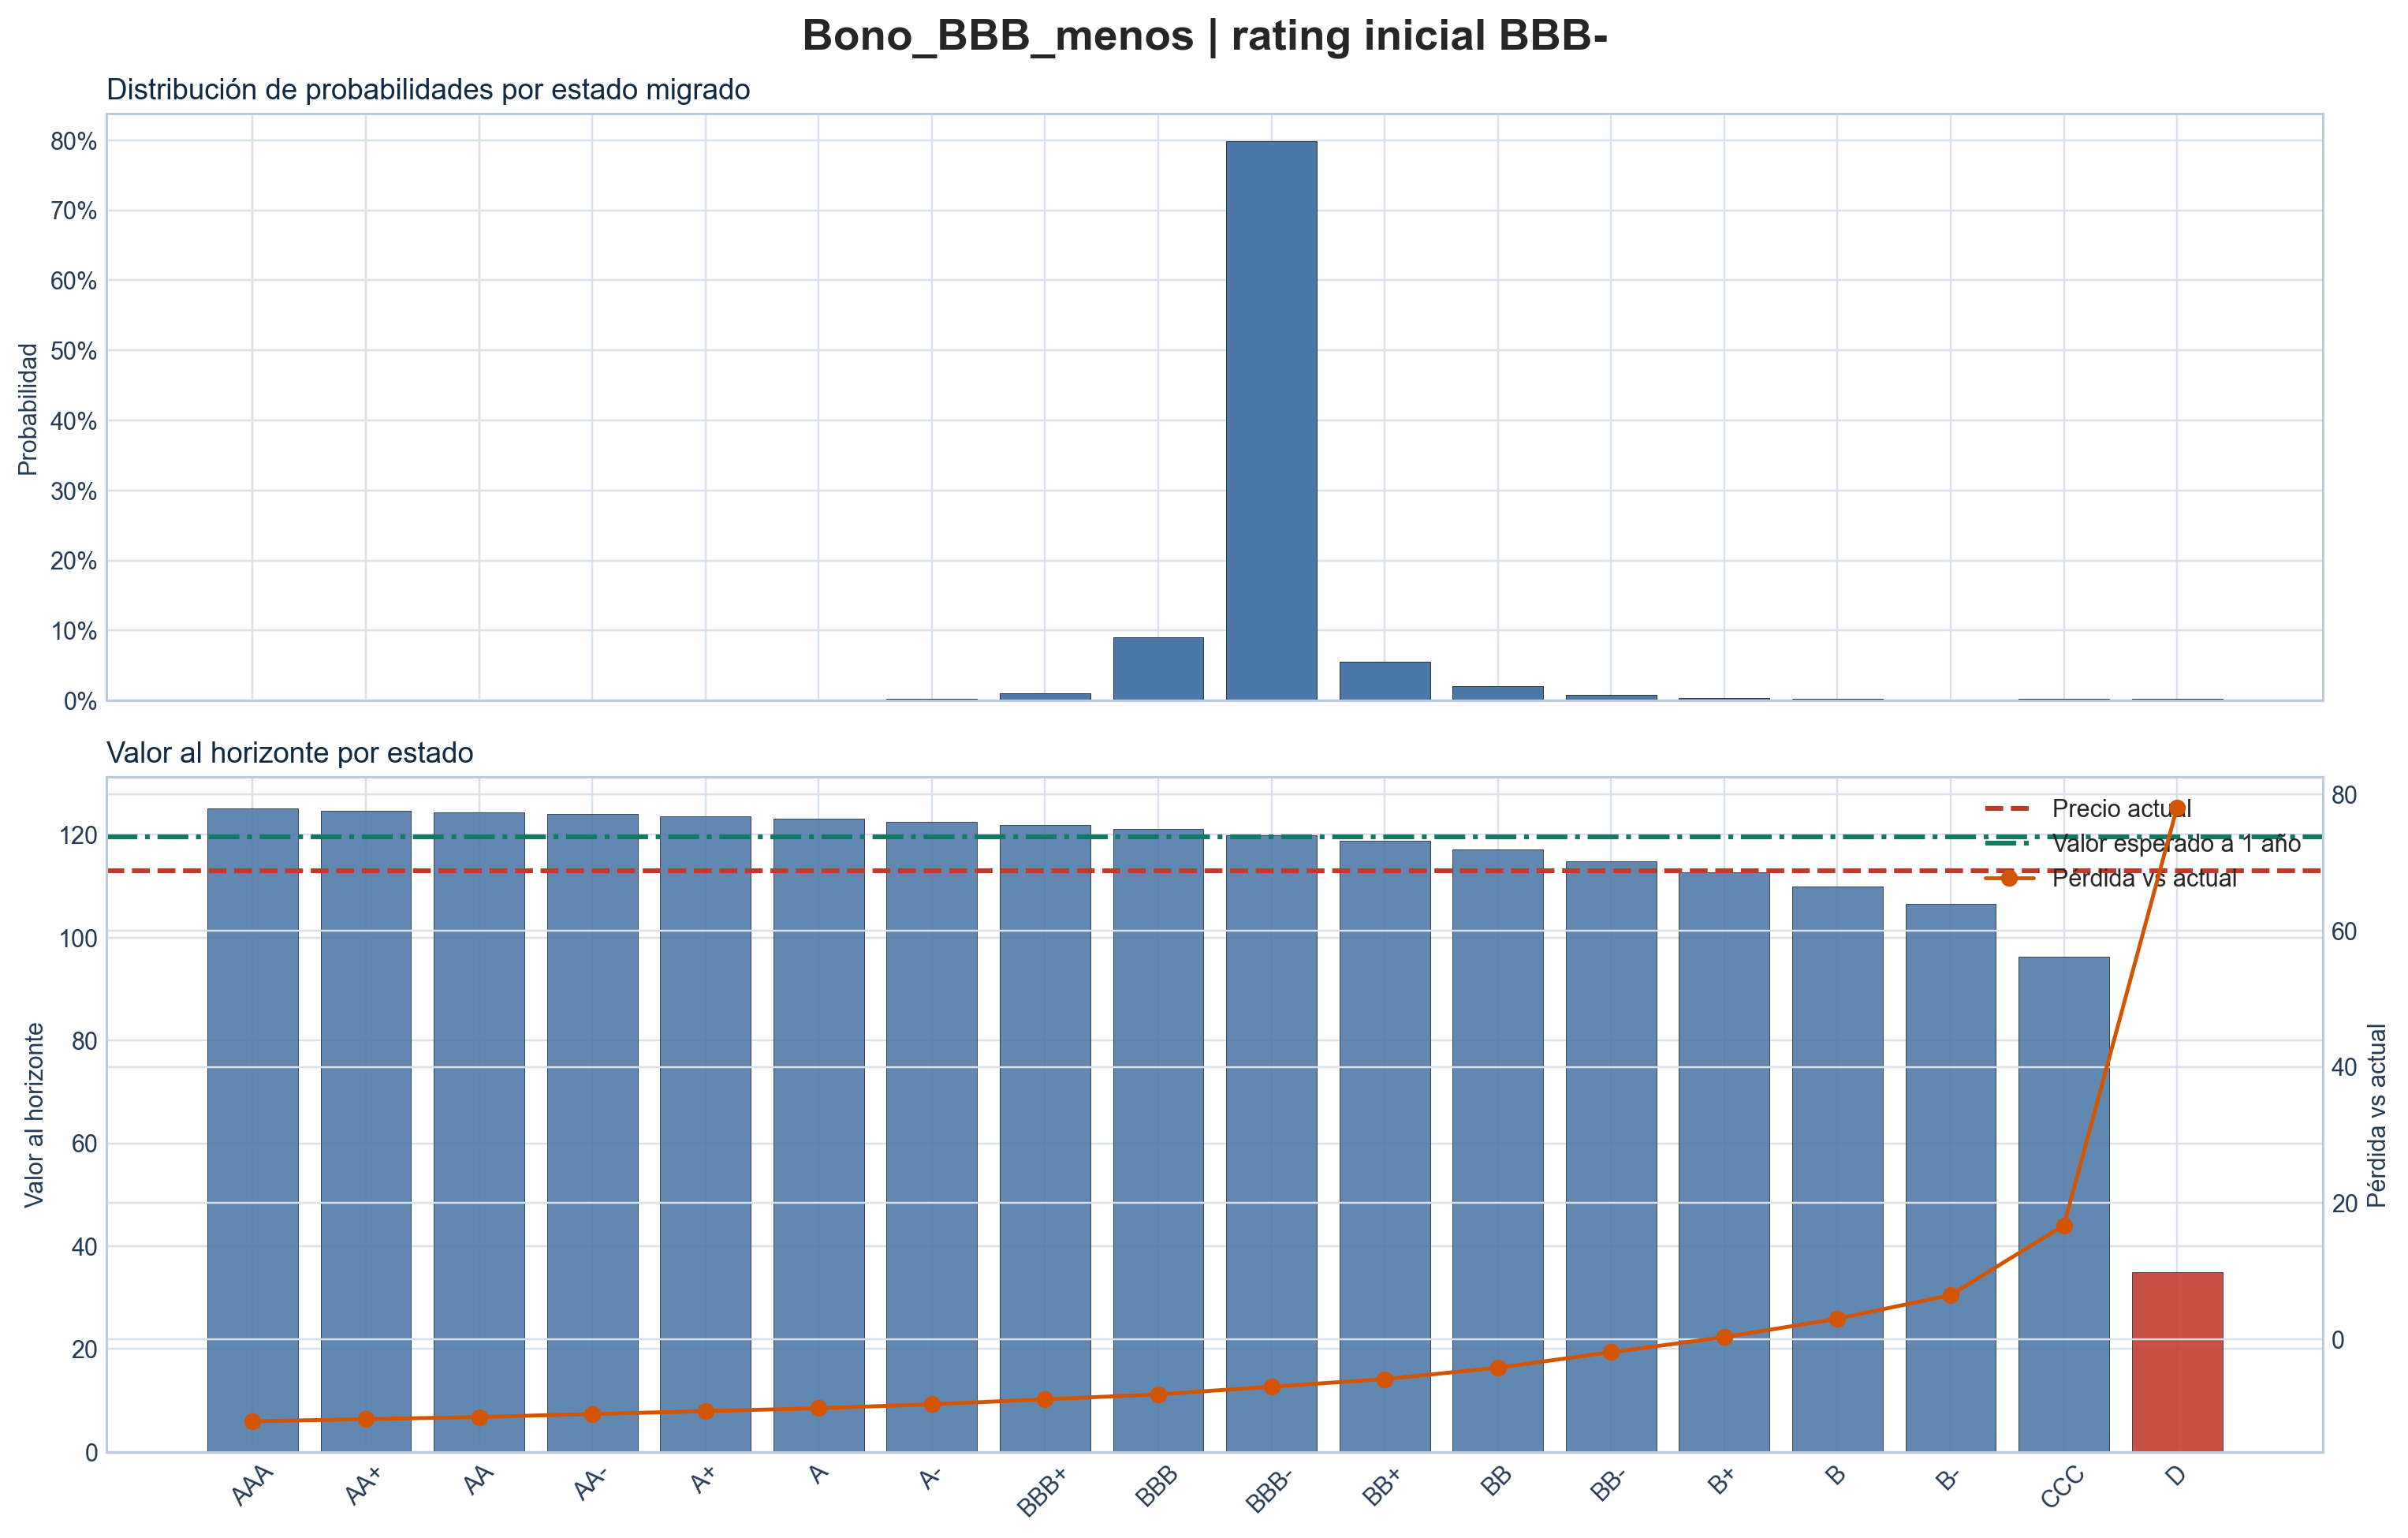
\includegraphics[width=\textwidth]{04_grafica_bono_bbb_menos.png}
\caption{Distribuci\'on de probabilidad y valor al horizonte para el bono BBB-.}
\end{figure}

En el bono BBB- aparece una combinaci\'on m\'as delicada: el valor esperado sigue siendo alto, pero la cola de p\'erdidas crece de forma visible. Su VaR individual es elevado porque el default produce una ca\'ida marcada respecto al precio actual.

\begin{figure}[H]
\centering
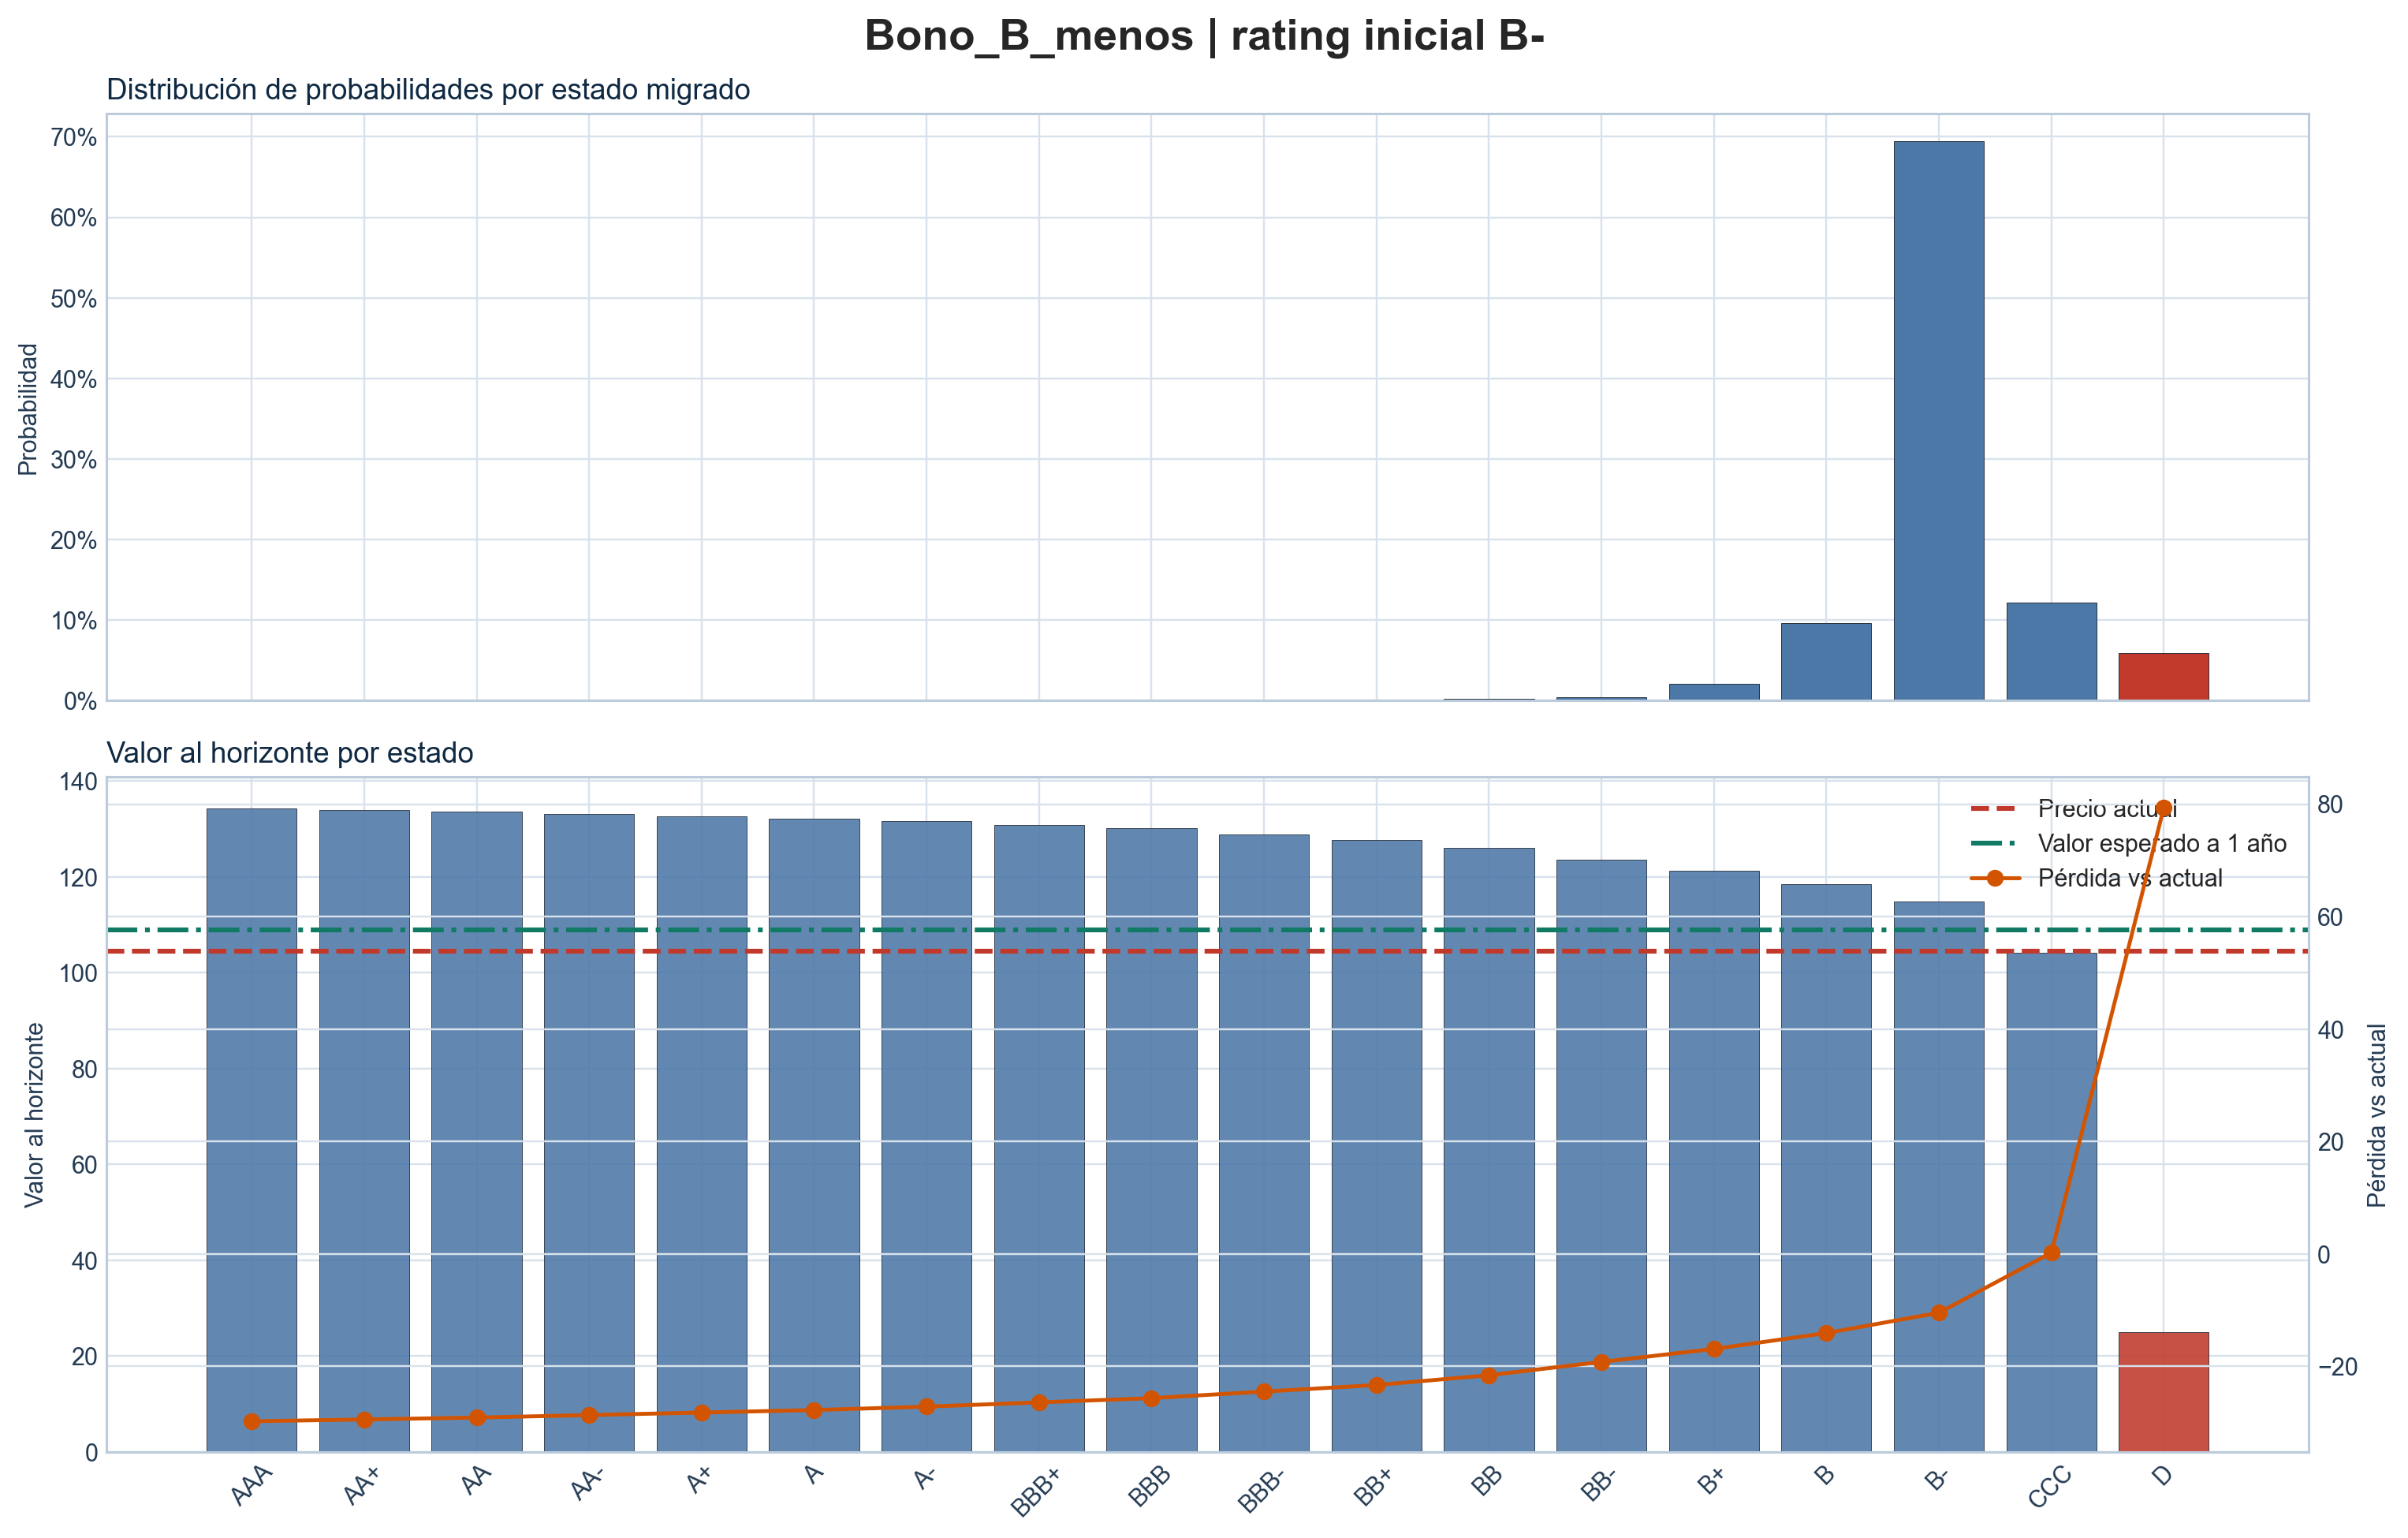
\includegraphics[width=\textwidth]{05_grafica_bono_b_menos.png}
\caption{Distribuci\'on de probabilidad y valor al horizonte para el bono B-.}
\end{figure}

El bono B- es el activo m\'as riesgoso del portafolio. La probabilidad de deterioro severo y default es sustancialmente mayor, y eso se traduce en la mayor volatilidad individual del conjunto.

\section*{Distribuci\'on del portafolio}

\begin{figure}[H]
\centering
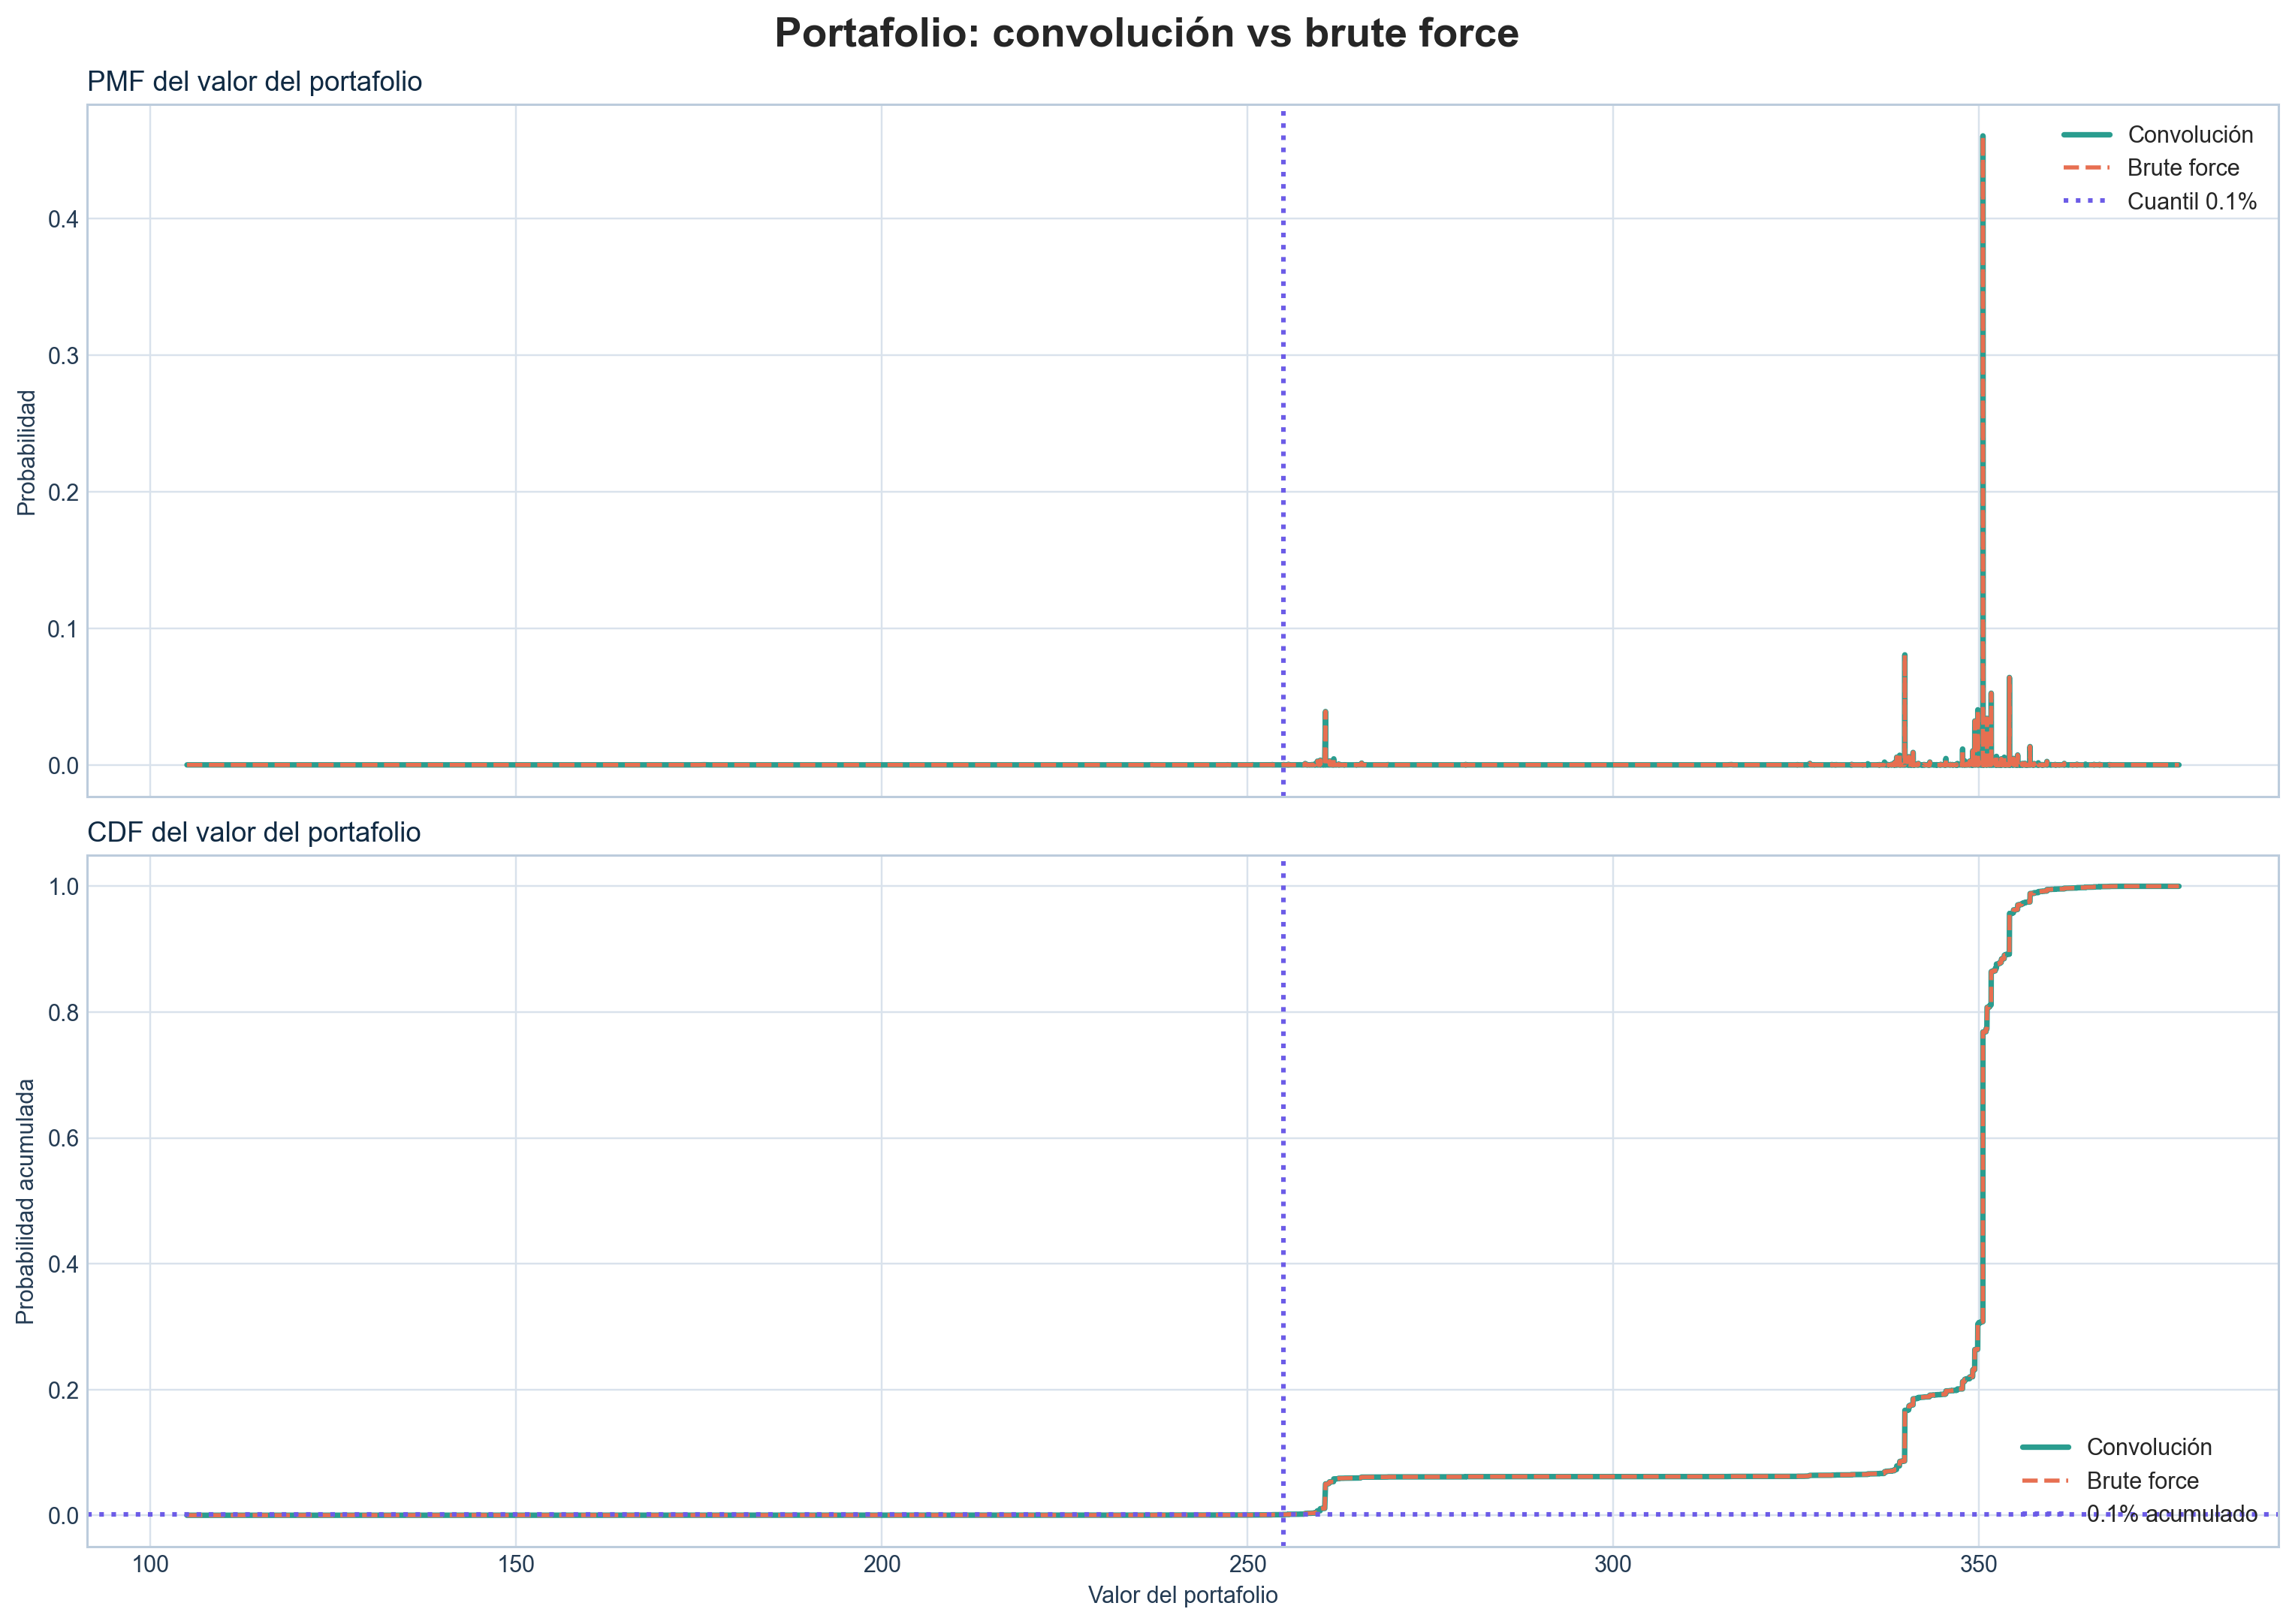
\includegraphics[width=\textwidth]{06_grafica_portafolio_distribucion.png}
\caption{PMF y CDF del portafolio: convoluci\'on vs brute force.}
\end{figure}

La superposici\'on entre ambas curvas muestra que la convoluci\'on reproduce exactamente la distribuci\'on obtenida por enumeraci\'on completa a nivel centavos. Adem\'as, el cuantil inferior del 0.1\% se ubica alrededor de \LowerTail, lo que equivale a una p\'erdida de aproximadamente \PortfolioVaR\ respecto al valor actual.

\begin{figure}[H]
\centering
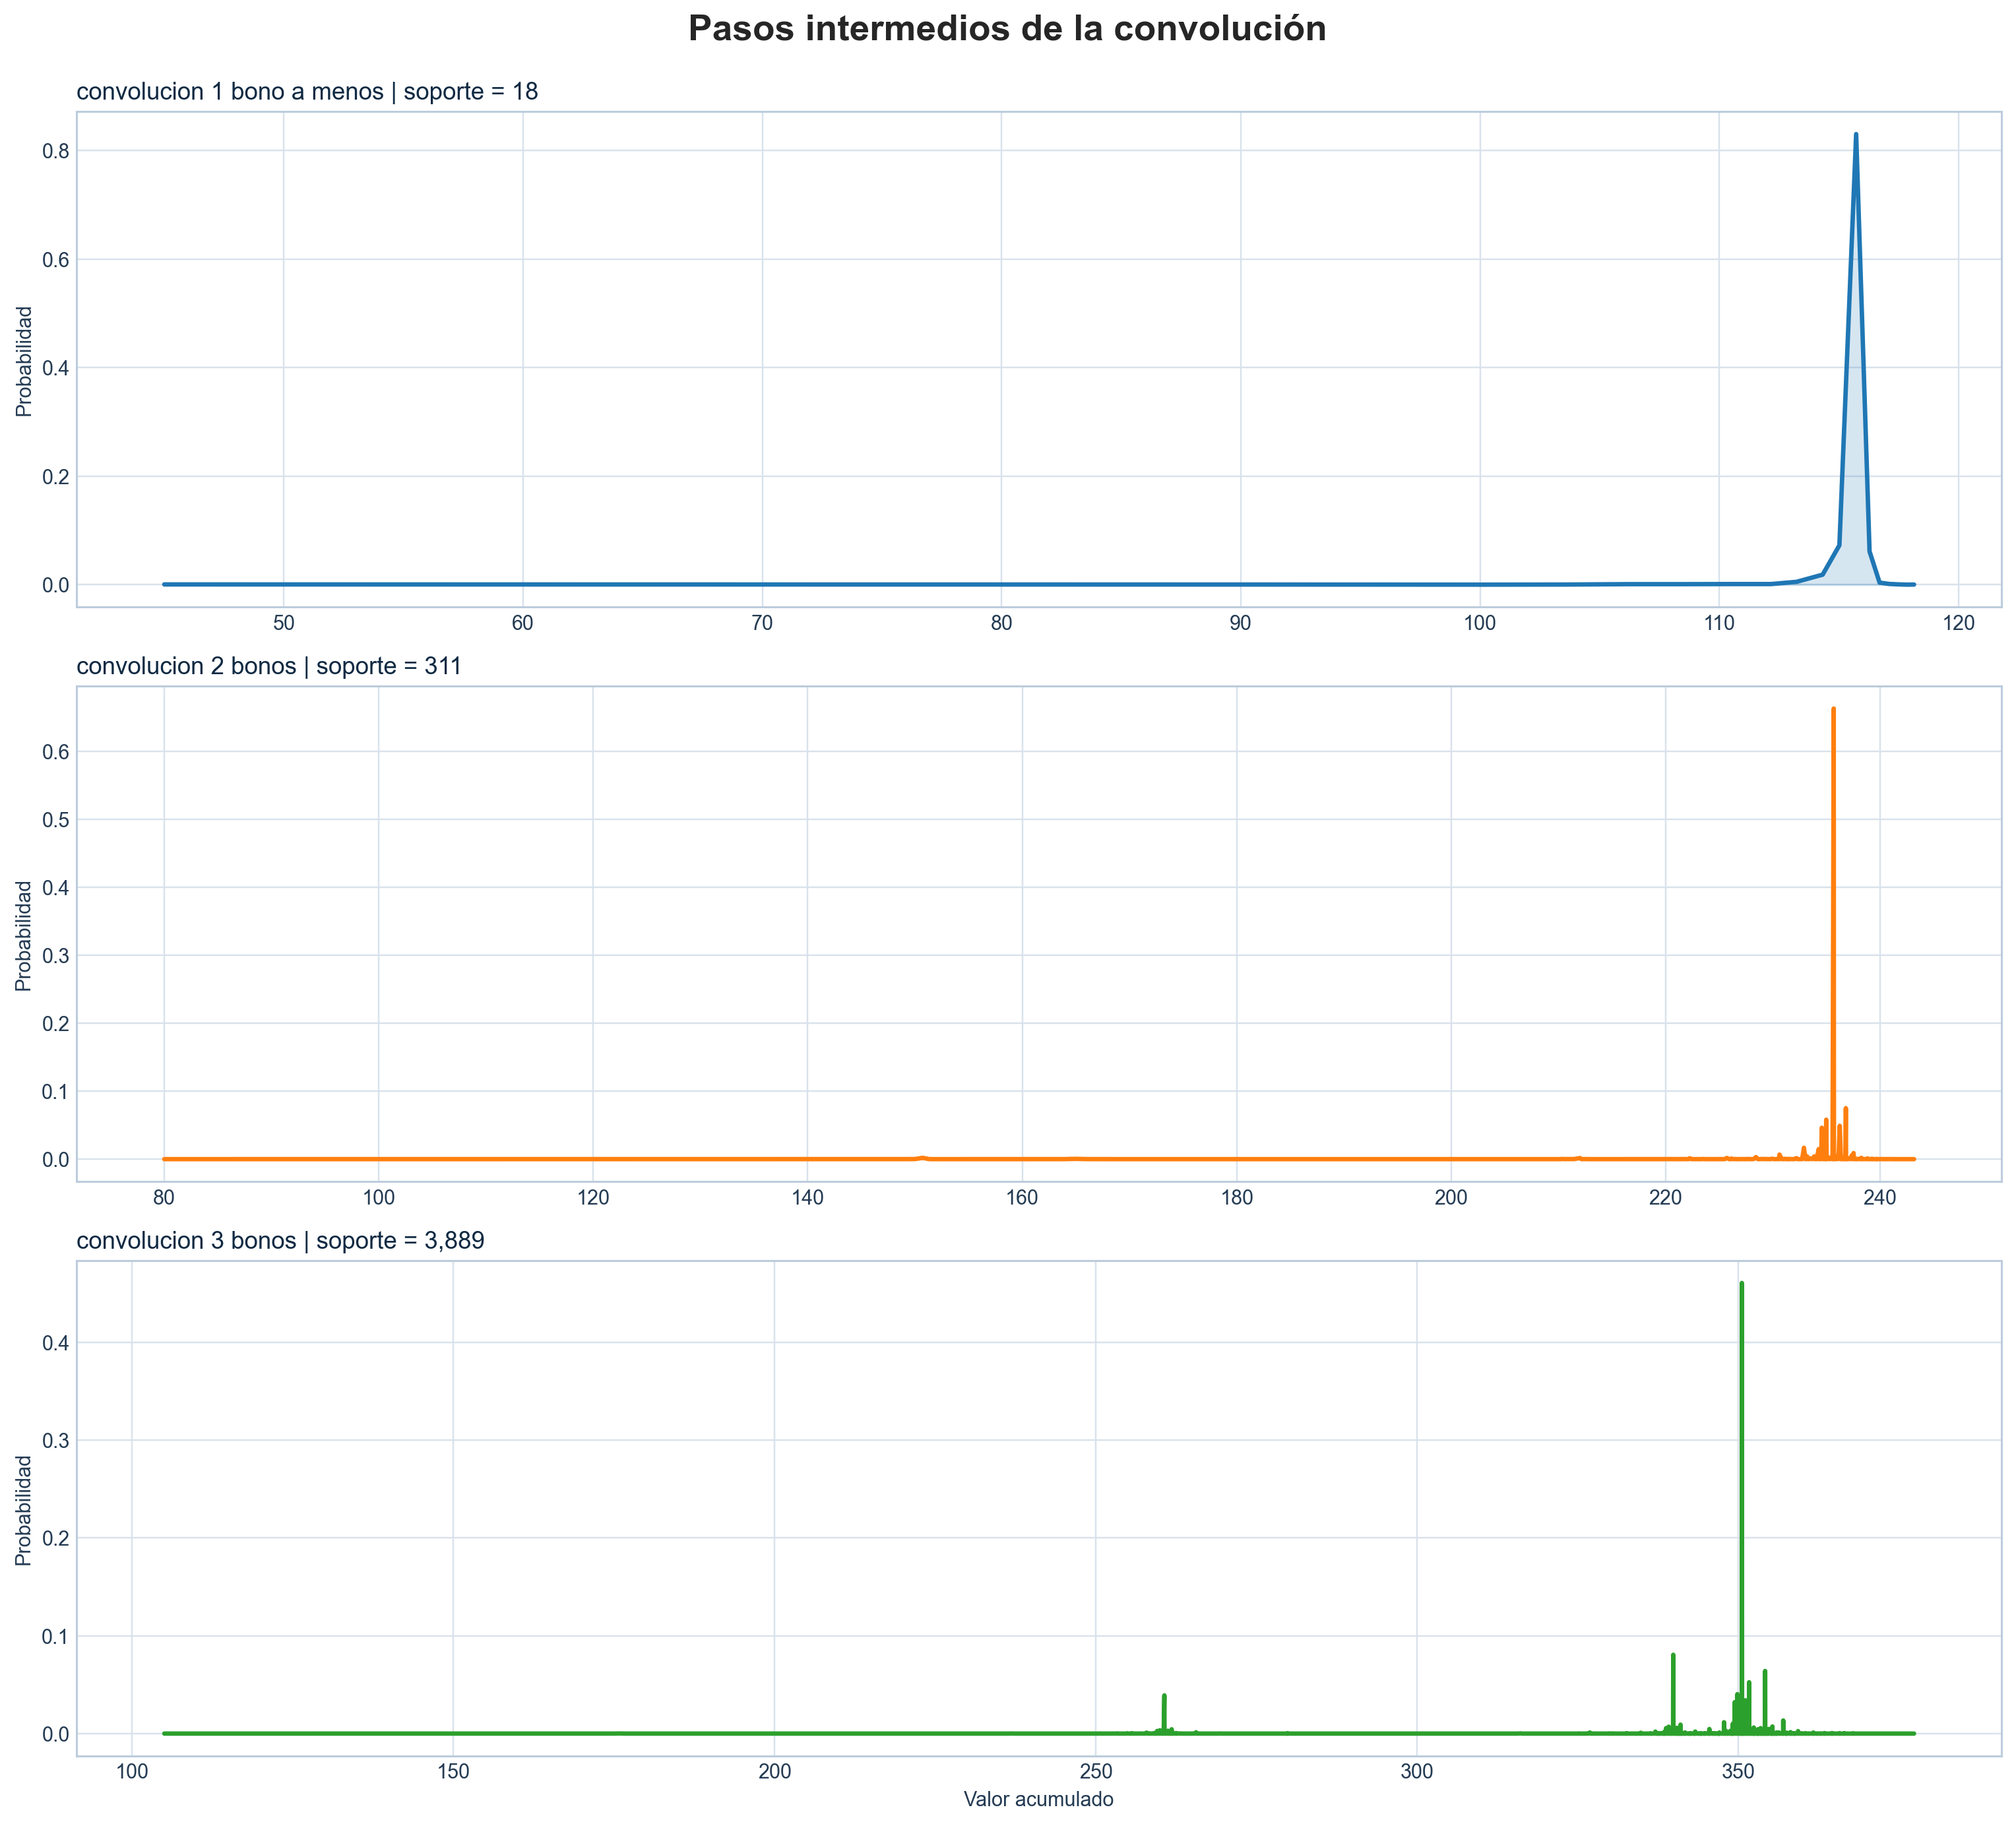
\includegraphics[width=\textwidth]{07_grafica_pasos_convolucion.png}
\caption{Pasos intermedios de la convoluci\'on.}
\end{figure}

Esta figura es importante porque muestra que la distribuci\'on del portafolio se construye de forma incremental: primero se toma el soporte del primer bono, luego se suma el segundo y finalmente el tercero. El soporte crece, pero sin necesidad de mantener una tabla manual de los \(5{,}832\) escenarios.

\section*{Tablas visuales para el reporte}

\begin{figure}[H]
\centering
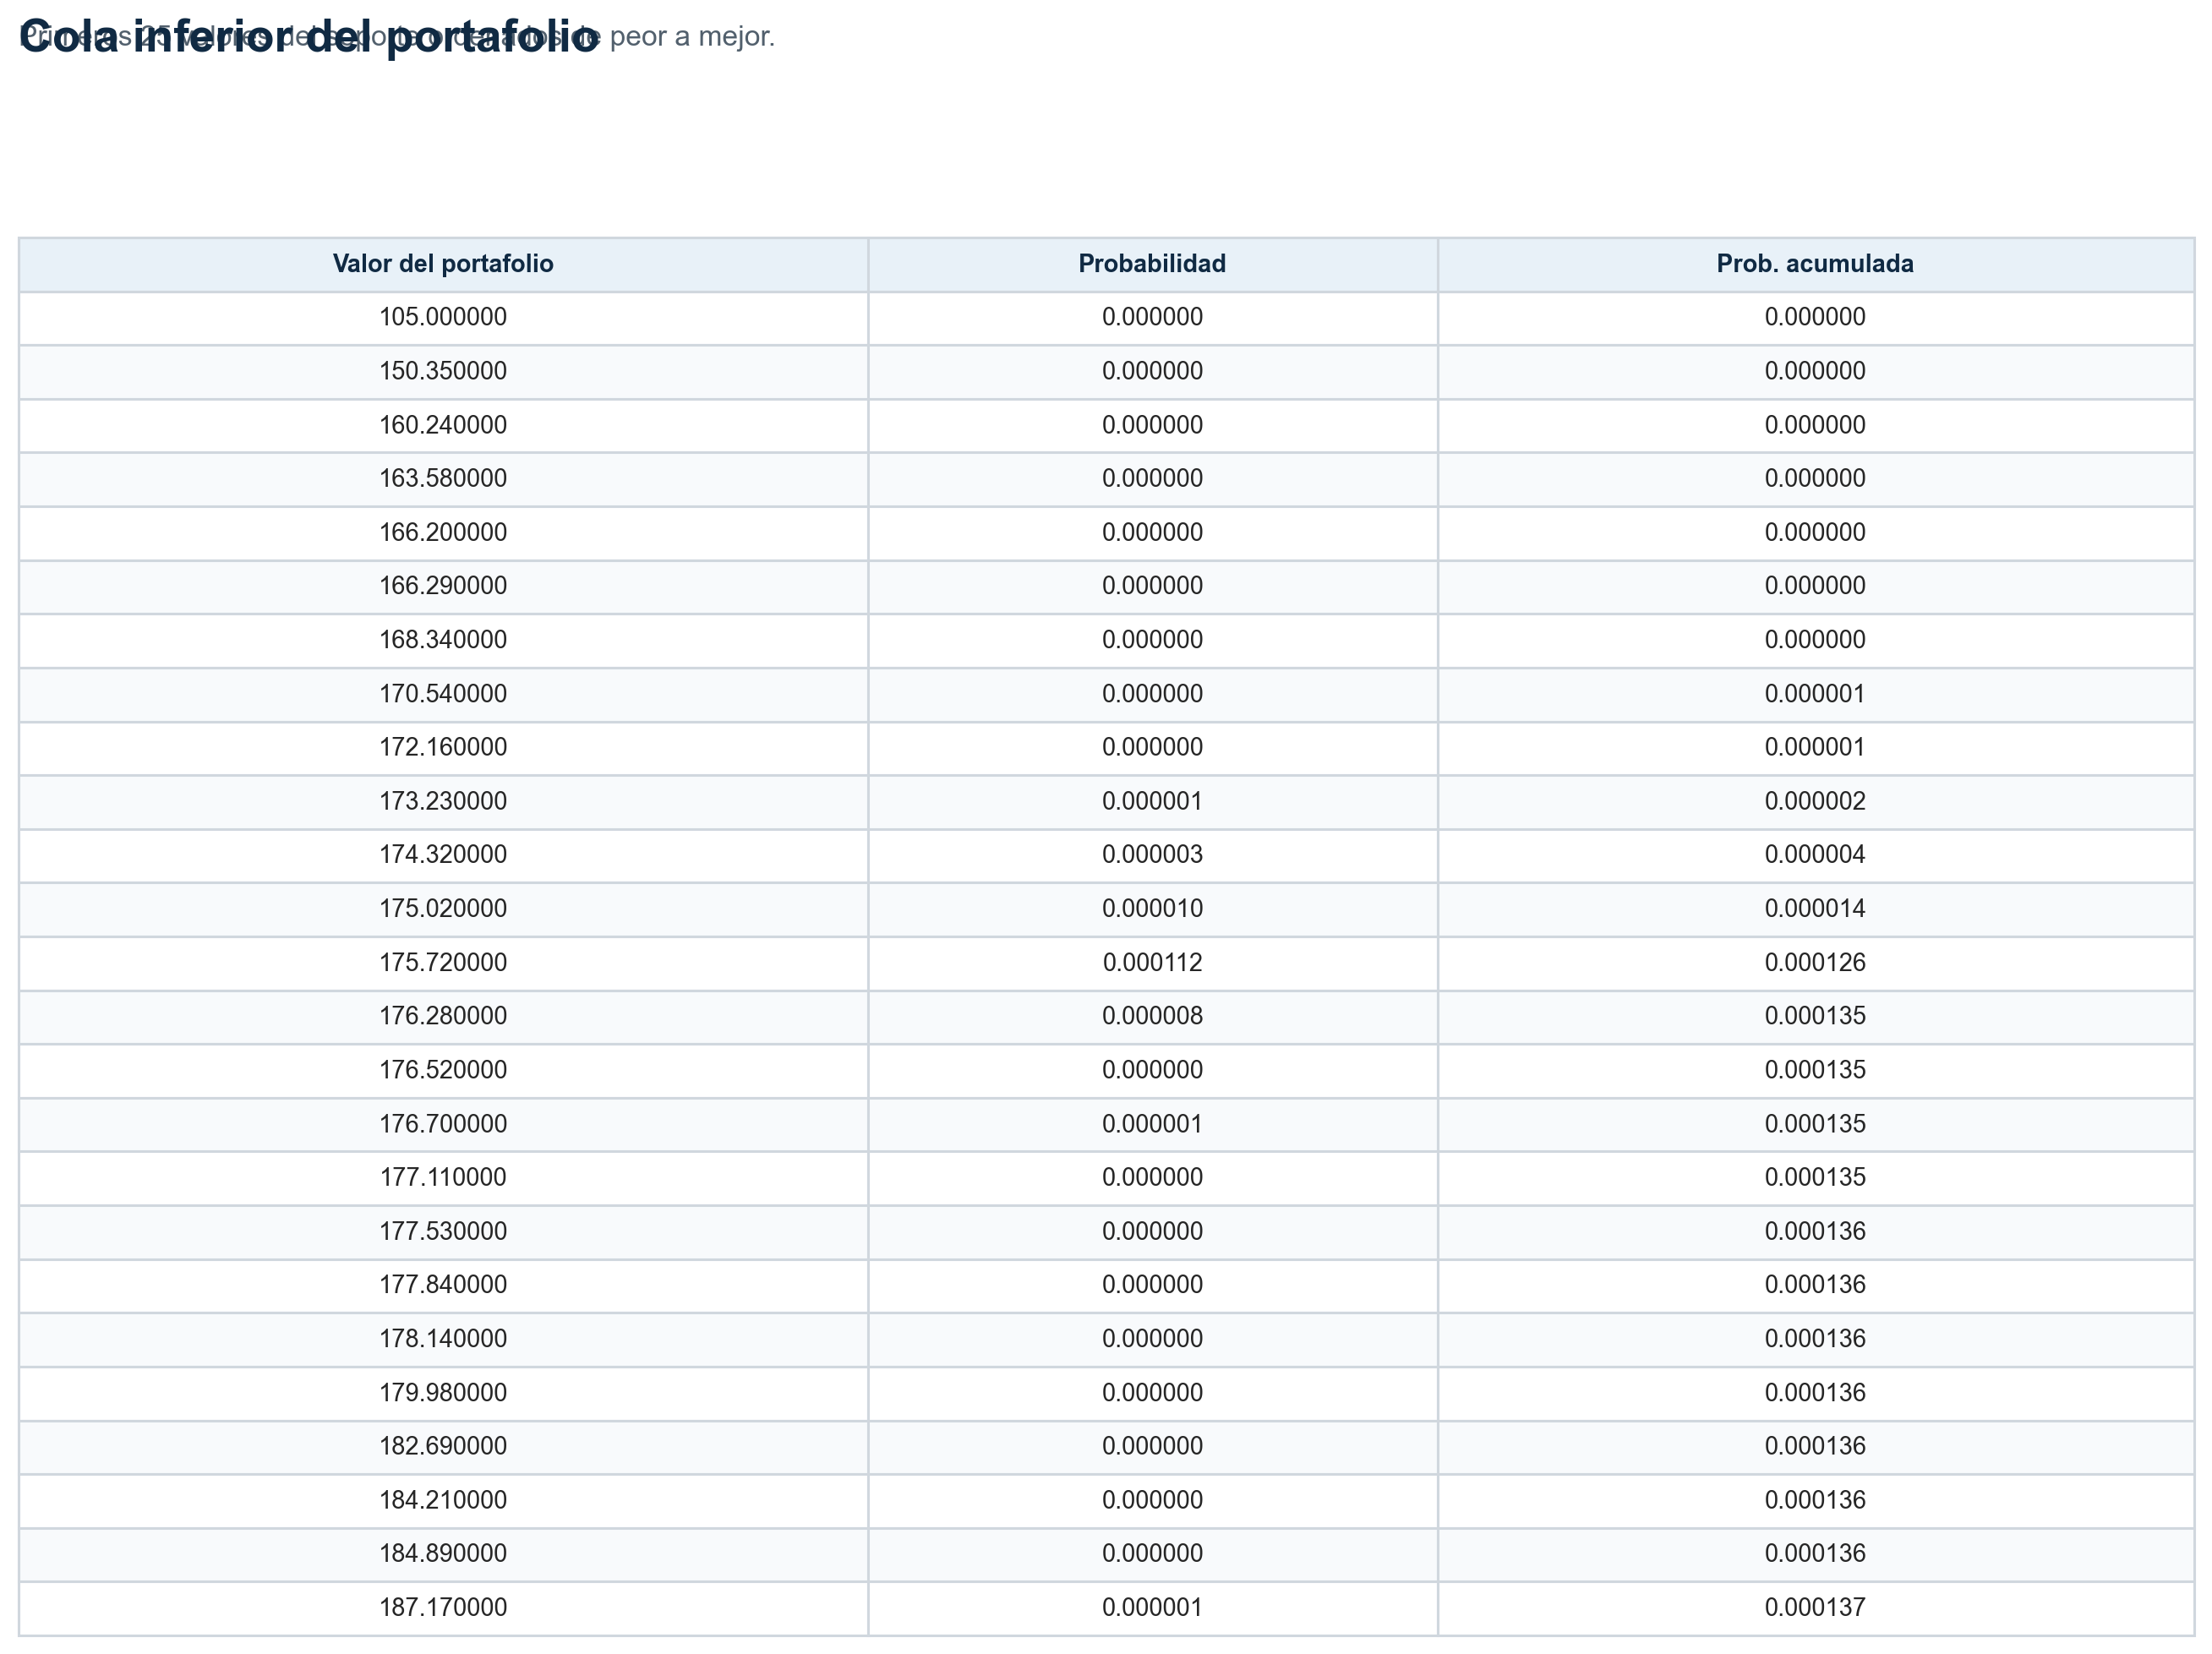
\includegraphics[width=\textwidth]{08_tabla_cola_portafolio.png}
\caption{Cola inferior del portafolio ordenada por valor.}
\end{figure}

La cola inferior concentra los peores valores del portafolio. Es la parte relevante para VaR y ES, porque all\'i viven los escenarios de estr\'es m\'aximo.

\begin{figure}[H]
\centering
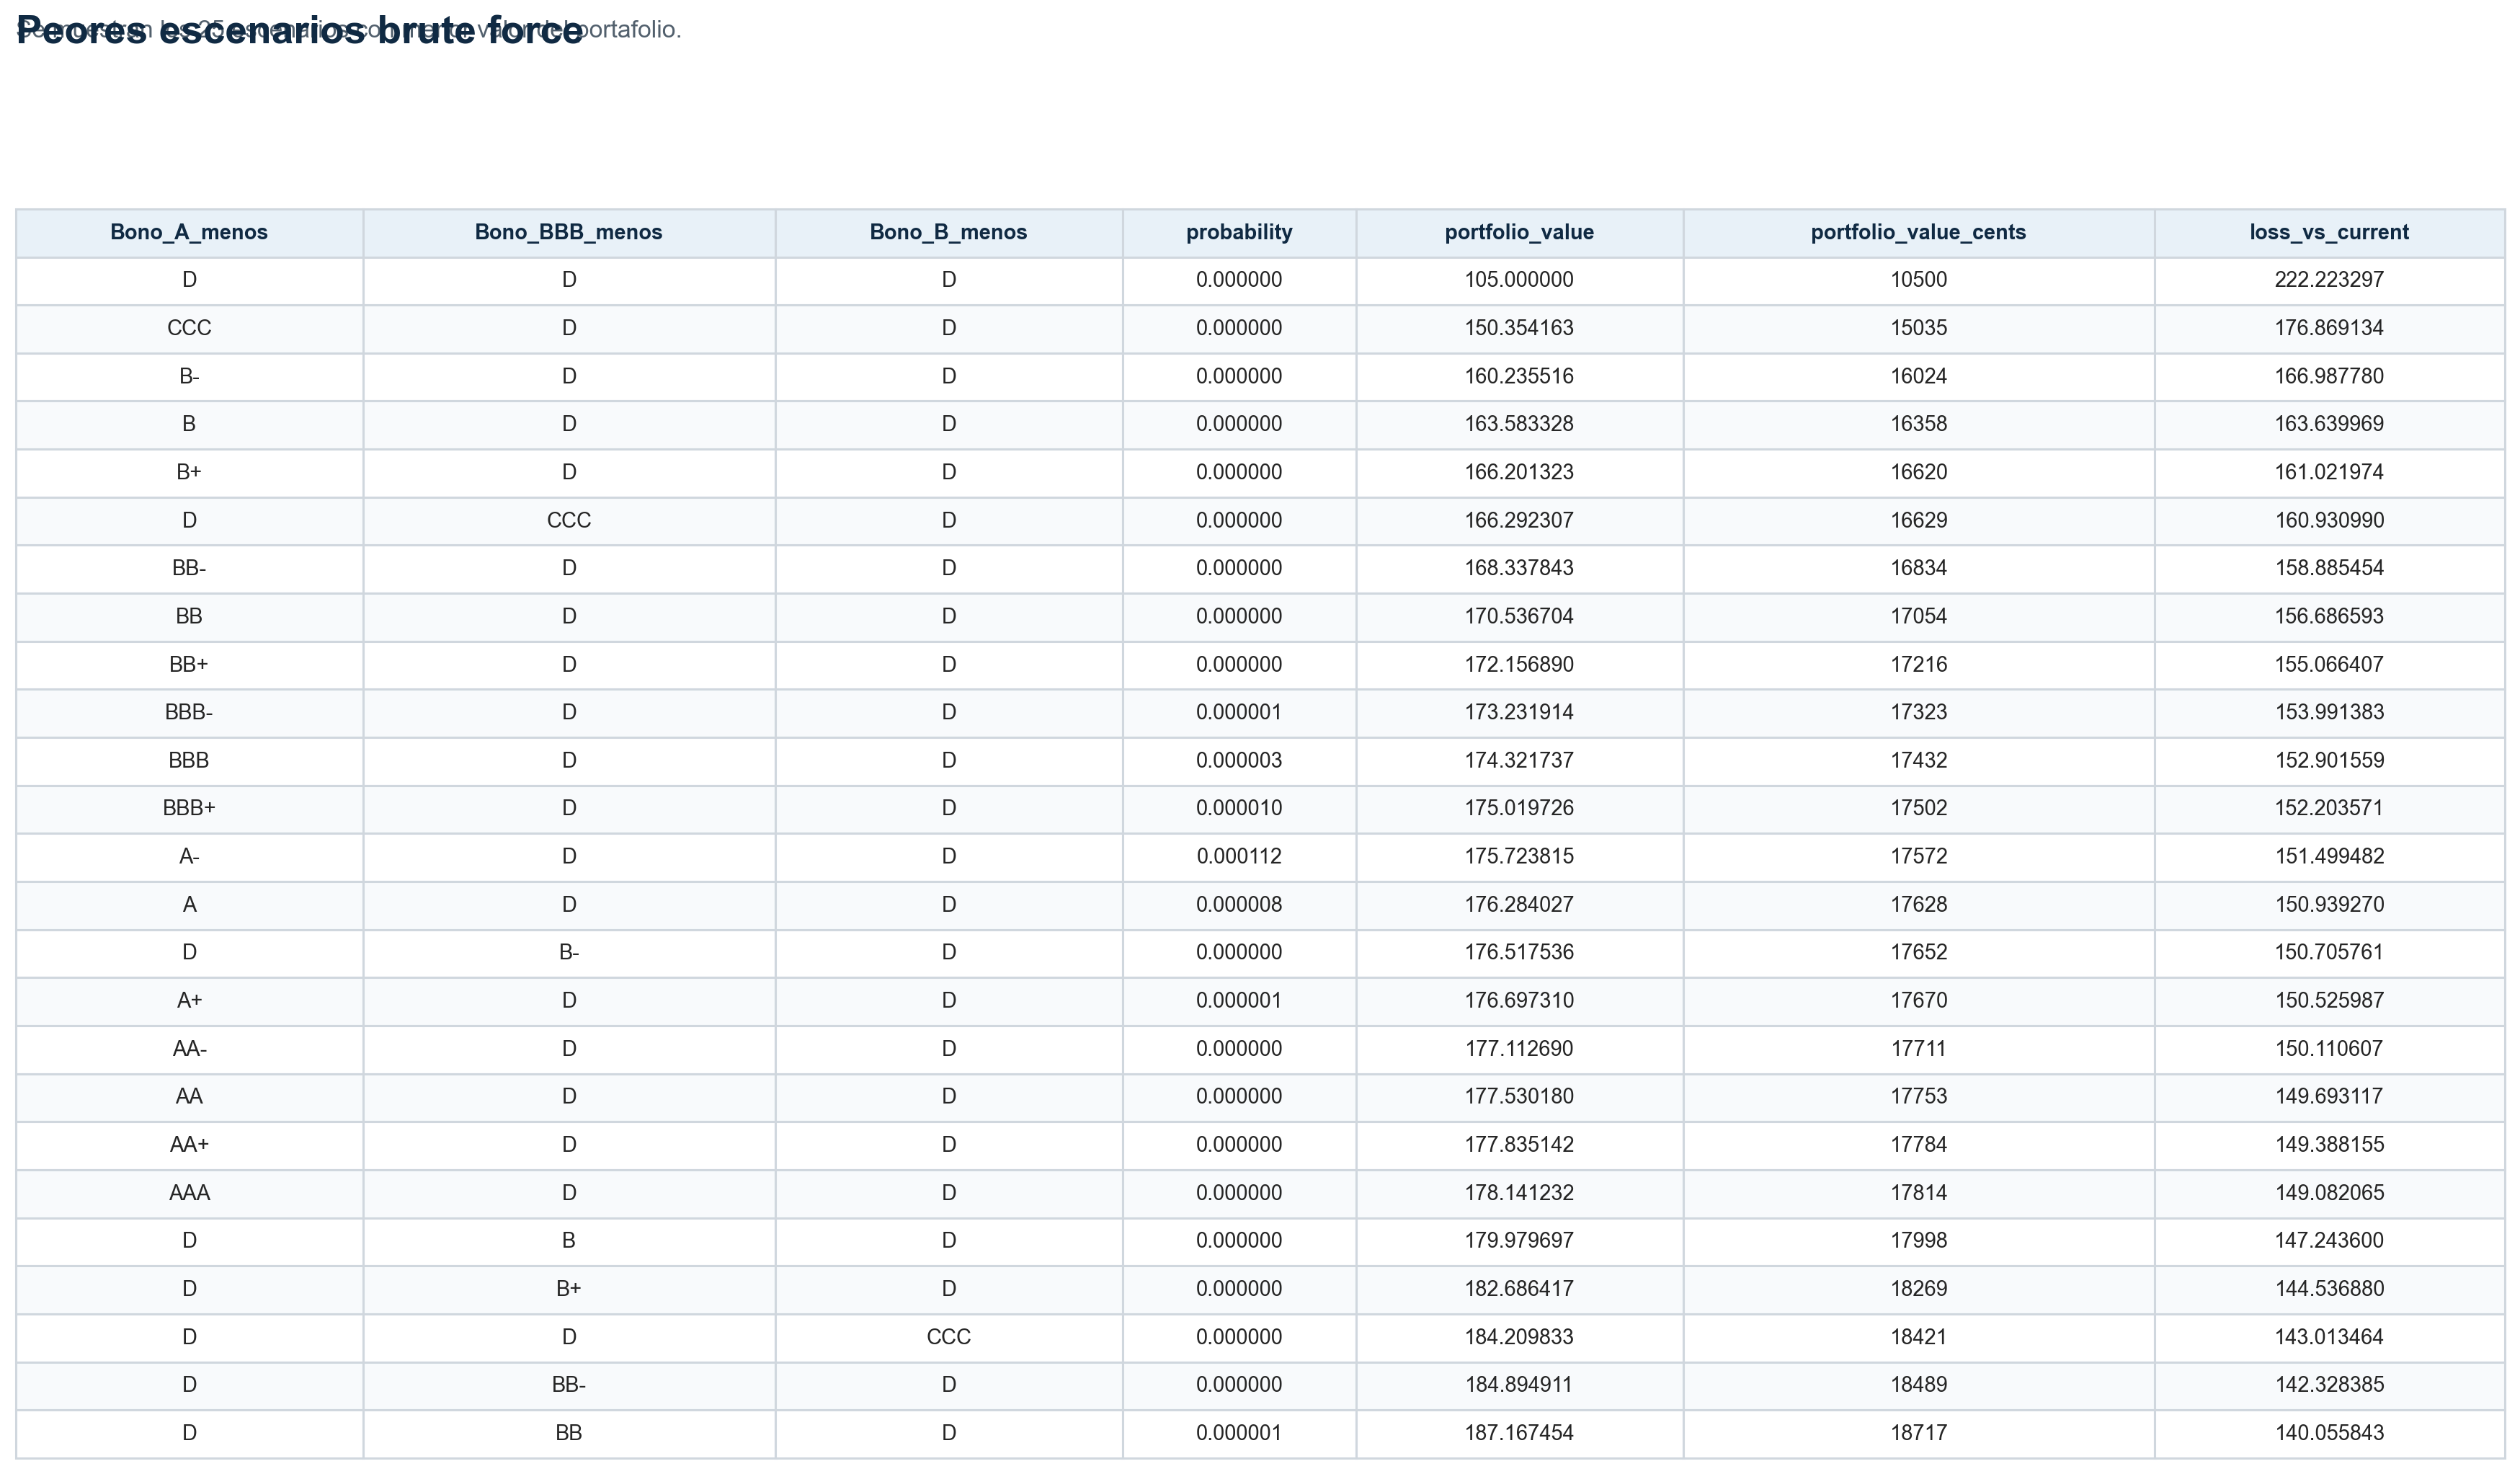
\includegraphics[width=\textwidth]{09_tabla_peores_escenarios_bruteforce.png}
\caption{Peores escenarios obtenidos por brute force.}
\end{figure}

Los peores escenarios muestran que el riesgo extremo no proviene del bono A-, sino de eventos severos en los bonos BBB- y B-. El escenario umbral reportado por el modelo es \texttt{\ThresholdScenario}, que combina estabilidad relativa del bono A- con deterioro extremo en los bonos m\'as riesgosos.

\begin{figure}[H]
\centering
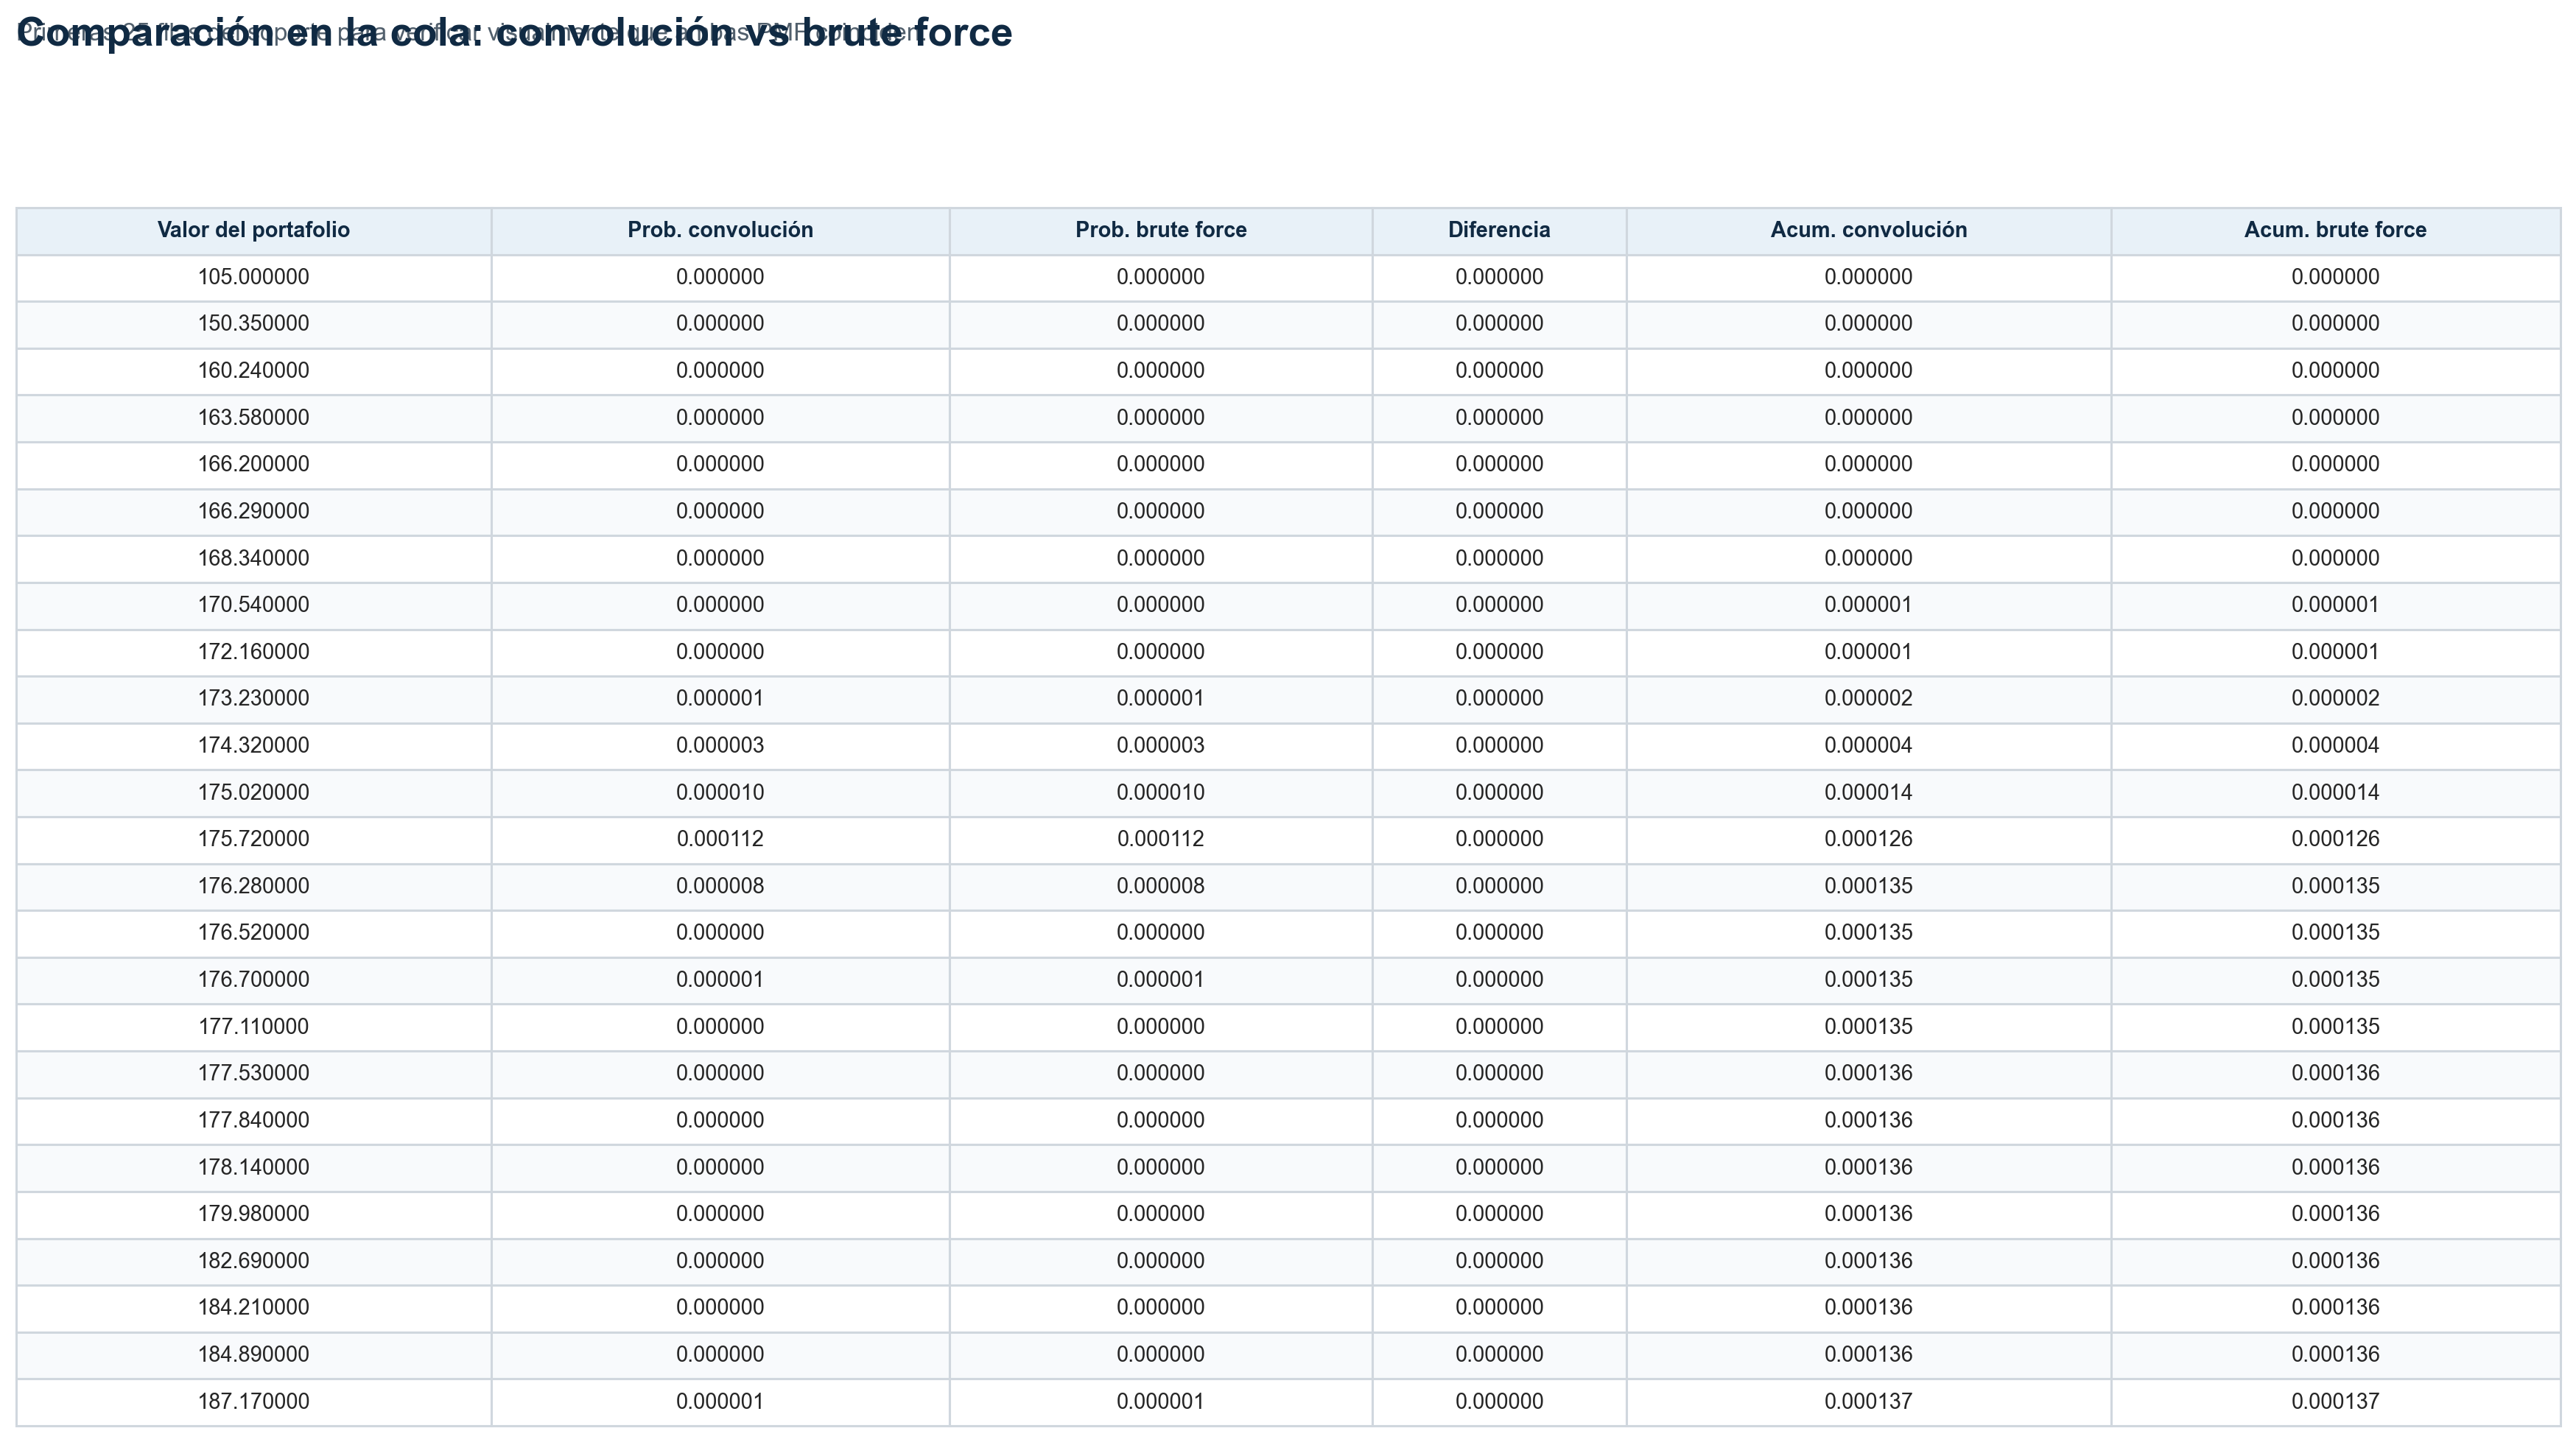
\includegraphics[width=\textwidth]{10_tabla_comparacion_convolucion_vs_bruteforce.png}
\caption{Comparaci\'on fila a fila entre convoluci\'on y brute force en la cola.}
\end{figure}

La comparaci\'on visual de la cola sirve como evidencia metodol\'ogica: la diferencia entre ambas PMF es nula o despreciable al nivel de redondeo usado por el proyecto.


\chapter{Interpretaci\'on financiera}
Desde el punto de vista financiero, el resultado principal del portafolio tiene una lectura clara.

\section*{1. La p\'erdida esperada es negativa}

La p\'erdida esperada del portafolio es \ExpectedLoss. En este contexto, un valor negativo no significa que el modelo est\'e mal; significa que, en promedio, el carry de los cupones y el rendimiento esperado a 1 a\~no superan la p\'erdida media por deterioro crediticio.

\section*{2. El riesgo extremo sigue siendo material}

Aunque el promedio es favorable, la cola izquierda sigue siendo pesada. El VaR 99.9\% es \PortfolioVaR\ y el ES 99.9\% es \PortfolioES. Eso implica que:

\begin{itemize}
  \item en el cuantil 99.9\%, la p\'erdida no excede aproximadamente \PortfolioVaR;
  \item pero si se entra en la cola m\'as extrema, la p\'erdida promedio sube hasta alrededor de \PortfolioES.
\end{itemize}

En otras palabras, el portafolio gana en promedio, pero est\'a expuesto a eventos raros con impacto considerable.

\section*{3. La mayor parte del riesgo no viene del bono A-}

La evidencia visual y los res\'umenes por bono indican que:

\begin{itemize}
  \item el bono A- tiene baja volatilidad y una distribuci\'on relativamente compacta;
  \item el bono BBB- contribuye de forma importante a la cola por su sensibilidad a migraciones severas y default;
  \item el bono B- es el principal generador de volatilidad y de escenarios extremos.
\end{itemize}

\section*{4. La convoluci\'on s\'i es una herramienta adecuada}

El c\'odigo demuestra algo metodol\'ogicamente valioso: en este ejercicio, la convoluci\'on no solo es m\'as c\'omoda que la enumeraci\'on completa, sino que reproduce exactamente el mismo resultado una vez que se trabaja a nivel centavos.

Eso significa que:

\begin{itemize}
  \item no se pierde precisi\'on relevante para el trabajo;
  \item se gana claridad computacional;
  \item se obtiene una validaci\'on robusta contra \textit{brute force}.
\end{itemize}

\section*{5. Interpretaci\'on final}

La lectura ejecutiva del portafolio es la siguiente:

\begin{itemize}
  \item el portafolio tiene carry positivo esperado;
  \item el riesgo de cola sigue siendo importante por la exposici\'on a bonos de menor calidad crediticia;
  \item el escenario umbral \texttt{\ThresholdScenario} muestra que una sola migraci\'on extrema puede dominar el comportamiento del portafolio;
  \item la implementaci\'on del repositorio es consistente con la teor\'ia de CreditMetrics y queda bien documentada para fines acad\'emicos o laborales.
\end{itemize}


\end{document}
